\documentclass[10pt]{book}
\usepackage[utf8]{inputenc}
\usepackage{geometry}
\usepackage{ngerman}
\usepackage[right]{eurosym}
\usepackage{titlesec}
\usepackage{graphicx}
\usepackage{caption}
\usepackage{flowfram}
\usepackage{tikz}
\usepackage{textpos}
\usepackage{calc}
\usepackage{amsmath, amssymb}
\usepackage{lastpage}
\usepackage{float}
\usepackage{ifthen}
\usepackage{changepage}
\usepackage{pgfplots}
\usepackage{sectsty}
\usepackage{tikz,xcolor,mwe}
\usepackage{booktabs,xcolor,siunitx}

\usetikzlibrary{arrows,
		calc,
		shadows,
		decorations.markings}

\definecolor{cvgreen}{HTML}{92D14F}
\definecolor{cvgray}{HTML}{D8E4BE}
\definecolor{cvtext}{HTML}{000000}
\definecolor{cvtabt}{HTML}{e5e2cc}

\definecolor{lightgray}{gray}{0.9}

\pgfplotsset{compat=1.9}

\newcommand\titelpage{%
\thispagestyle{empty}
\begin{tikzpicture}[overlay, remember picture]
    % green bar
    \fill[cvgreen] (current page.north west) rectangle ([xshift=5cm]current page.south west);
    % gray bar
    \fill[cvgray] ([yshift=-5cm]current page.north west) rectangle ([yshift=-10cm]current page.north east);
    % title and date
    \node[cvtext,right] at ([xshift=1.5cm,yshift=-7cm]current page.north west) {\Huge\bfseries Mathe-Notizen für Selbstudium};
    \node[cvtext,right] at ([xshift=1.5cm,yshift=-8cm]current page.north west) {\Huge 1. Auflage};
    \node[cvtext,above left] at ([xshift=-1cm,yshift=-8.5cm]current page.north east) {\Huge\bfseries vom \today };
    % cover photo
    \node[inner sep=0pt,below right] (image) at ([xshift=5cm,yshift=-5cm]current page.north west)
    {
\includegraphics[width=11cm,height=15cm]{./pics/me}};
    % name and address
    \node[fill=white,align=center,text width=6.4cm,inner sep=0.3cm,below] (name) at (image.south)
        {\LARGE Jens Kallup};
    \node[text width=15cm,inner sep=0.3cm,below right] at (name.south west) {\Large\obeylines%
        Langensalzer Str. 30\\
        99817 Eisenach\\
        Tel.: 03691 / \\
        E-Mail: kallup.jens@web.de
    };
    % attachments
    \node[black,text width=5cm,inner sep=0.3cm,above right] at ([yshift=1cm]current page.south west) {\large\obeylines%
        \textbf{Inhalt:}\\[4pt]
        Eigene Gedanken zu:\\[3pt]
        de.sci.mathematik \\
        de.sci.informatik
    };
\end{tikzpicture}
}


\titleformat{name=\chapter}[display]{\Huge\bfseries\sffamily\color{white}}{%
\thispagestyle{empty}
\begin{tikzpicture}[overlay, remember picture]
        \path let \p1 = (current page.west), \p2 = (current page.east) in
        node[minimum width=\x2-1.5pt, minimum height=4cm,
        rectangle, fill=cyan, anchor=north west, align=left, text width=\x2-\x1] at ($(current page.north west)$) {
        \begin{textblock*}{5in}(\dimexpr\x2-4.0in,\dimexpr0.25\headheight-1in)
          \tikz \node [white,text width=2in, align=right, font=\sffamily] {{\normalsize MATHEMATIK }\\[10pt]
          \raisebox{20pt}{{\large \chaptertitlename}} \raisebox{-12pt}{\chapternumberfont \thechapter}};
        \end{textblock*}};
        \path let \p1 = (current page.west), \p2 = (current page.east) in
              node[minimum width=\x2-\x1, minimum height=-2.8in, rectangle, fill=cyan!50, anchor=south west, align=left, text width=\x2-\x1] at ($(current page.south west)$) {\textcolor{black}{\Large{\thepage . \: \: de.sci.mathematik}}};
\end{tikzpicture}}{-1.75in}{}[\vspace*{0.25in}]


\titleformat{name=\chapter,numberless}[display]{\Huge{\bfseries\sffamily\color{yellow}}}{%
   \thispagestyle{empty}
  \begin{tikzpicture}[overlay, remember picture]
     \path let \p1 = (current page.west), \p2 = (current page.east) in
     node[minimum width=\x2-1.5pt, minimum height=4cm,
     rectangle, fill=cyan, anchor=north west, align=left, text width=\x2-\x1] at ($(current page.north west)$) {
        \begin{textblock*}{5in}(\dimexpr\x2-4.0in,\dimexpr0.25\headheight-1in)
           \tikz \node [white,text width=2in, align=right, font=\sffamily] {{\normalsize MATHEMATIK }\\[10pt]
           \raisebox{20pt}{{\large \chaptertitlename}} \raisebox{-12pt}{\chapternumberfont \thechapter}};
     \end{textblock*}
  };
     \fill[cyan](current page.south west) rectangle ($(current page.south east) - (0,-1.5cm)$);
\end{tikzpicture}}{-1.75in}{}[\vspace*{0.25in}]
 
\titleformat{name=\section}[display]{\Huge{\bfseries\sffamily\color{yellow}}}{%
   \thispagestyle{empty}
  \begin{tikzpicture}[overlay, remember picture]
     \path let \p1 = (current page.west), \p2 = (current page.east) in
     node[minimum width=\x2-1.5pt, minimum height=4cm,
     rectangle, fill=cyan, anchor=north west, align=left, text width=\x2-\x1] at ($(current page.north west)$) {
        \begin{textblock*}{5in}(\dimexpr\x2-4.0in,\dimexpr0.25\headheight-1in)
           \tikz \node [white,text width=2in, align=right, font=\sffamily]
           {\normalsize MATHEMATIK }\\[10pt];
        \end{textblock*}
  };
     \fill[cyan](current page.south west) rectangle ($(current page.south east) - (0,-1.5cm)$);
\end{tikzpicture}}{-1.75in}{}[\vspace*{0.25in}]
 
\titleformat{name=\subsection}{\Huge{\bfseries\sffamily\color{yellow}}}{%
   \thispagestyle{empty}
  \begin{tikzpicture}[overlay, remember picture]
     \path let \p1 = (current page.west), \p2 = (current page.east) in
     node[minimum width=\x2-1.5pt, minimum height=4cm,
     rectangle, fill=cyan, anchor=north west, align=left, text width=\x2-\x1] at ($(current page.north west)$) {
        \begin{textblock*}{5in}(\dimexpr\x2-4.0in,\dimexpr0.25\headheight-1in)
           \tikz \node [white,text width=2in, align=right, font=\sffamily] {{\normalsize MATHEMATIK }\\[10pt]
           \raisebox{20pt}{{\large \chaptertitlename}} \raisebox{-12pt}{\chapternumberfont \thechapter}};
     \end{textblock*}};
     \fill[cyan](current page.south west) rectangle ($(current page.south east) - (0,-1.5cm)$);
\end{tikzpicture}}{-1.75in}{}[\vspace*{0.25in}]
 
\titleformat{name=\subsubsection}[display]{\Huge{\bfseries\sffamily\color{yellow}}}{%
   \thispagestyle{empty}
  \begin{tikzpicture}[overlay, remember picture]
     \path let \p1 = (current page.west), \p2 = (current page.east) in
     node[minimum width=\x2-1.5pt, minimum height=4cm,
     rectangle, fill=cyan, anchor=north west, align=left, text width=\x2-\x1] at ($(current page.north west)$) {
        \begin{textblock*}{5in}(\dimexpr\x2-4.0in,\dimexpr0.25\headheight-1in)
           \tikz \node [white,text width=2in, align=right, font=\sffamily] {{\normalsize MATHEMATIK }\\[10pt]
           \raisebox{20pt}{{\large \chaptertitlename}} \raisebox{-12pt}{\chapternumberfont \thechapter}};
     \end{textblock*}};
     \fill[cyan](current page.south west) rectangle ($(current page.south east) - (0,-1.5cm)$);
\end{tikzpicture}}{-1.75in}{}[\vspace*{0.25in}]





\newcommand*\MyHeadBottom{%
\makeatletter
\strictpagecheck
\ifoddpage\else
\thispagestyle{empty}
\begin{tikzpicture}[overlay, remember picture]
\checkoddpage
	\path let \p1 = (current page.west), \p2 = (current page.east) in
        node[minimum width=\x2-1.5pt, minimum height=2cm,
        rectangle, fill=cyan, anchor=north west, align=left, text width=\x2-\x1] at ($(current page.north west)$) {
        \begin{textblock*}{5in}(\dimexpr\x2-4.0in,\dimexpr0.25\headheight-1cm)
          \tikz \node [white,text width=2in, align=right, font=\sffamily] {{\normalsize Neuronale Netze }\\[10pt]
                    \raisebox{20pt}{{\large \chaptertitlename}} \raisebox{-10pt}{\chapternumberfont \thechapter}};
        \end{textblock*}};
	\path let \p1 = (current page.west), \p2 = (current page.east) in
	              node[minimum width=\x2-\x1, minimum height=1cm, rectangle, fill=cyan!50, anchor=south west, align=right, text width=\x2-\x1] at
	        ($(current page.south west)$) {\textcolor{black}{\Large{\textbf{de.sci.mathematik \: \thepage . \: \:}}}};
\end{tikzpicture}
\fi
\makeatother
}

\newenvironment{MyConsoleBox}[1]
%BEGIN
{%
  \begingroup\setlength{\textwidth}{20cm}
  \colorbox{lightgray}{%
  \begin{tabular}{p{14.4cm}}
  #1
  \end{tabular}
  }\endgroup
}%
%END
{%
}


\newenvironment{MyTableBox}[1]
%BEGIN
{%
  \begingroup\setlength{\textwidth}{20cm}
  \colorbox{cvtabt}{%
  \begin{tabular}{|p{4cm}|p{5cm}|p{4cm}|}
  \hline
  #1
  \hline
  \end{tabular}
  }\endgroup
}%
%END
{%
}

\newcommand\bildzrange{%
\begin{tikzpicture}[overlay, remember picture]
   \node[inner sep=0pt,below right] (image) at ([xshift=-10cm,yshift=-3.1cm]current page.north east)
  {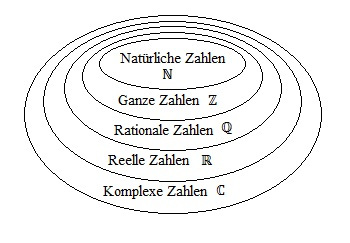
\includegraphics[width=7.5cm,height=4.1cm]{pics/zbereiche.jpg}};
\end{tikzpicture}}

\newcommand\legendezbereiche{%
\begin{tabular}{ll}
 $\mathbb{C}$  & = komplexe Zahl    \\
 $\mathbb{I}$  & = irrationale Zahl \\
 $\mathbb{N}$  & = natürliche Zahl  \\
 $\mathbb{Q}$  & = rationale Zahl   \\
 $\mathbb{R}$  & = reelle Zahl      \\
 $\mathbb{Z}$  & = ganze Zahl       \\
\end{tabular}
\\
\begin{tabular}{ll}
 $ f $         & = Funktion \\
 $ x $         & = Argument, x-Wert, unabhängige Variable  \\
 $ y $         & = Funktionswert, y-Wert, abhängige Variable  \\
 $ y = f(x) $  & = Funktionsgleichung, Zuordnungsvorschrift  \\
 $ f(x) $      & = spricht man ''f von x'' \\
 $ D \: (oder \: \mathbb{D} ) $ & = Definitionsmenge, Definitionsbereich  \\
 $ W $         & = Wertemenge, Wertebereich \\
 & \\
 $ f(x) = c $  & = konstante Funktion \\
 $ f(x) = mx + n $ & = lineare Funktion \\
 $ f(x) = ax^2 + bx + c $ & = quadratische Funktion \\
 $ f(x) = \frac{a_n x^a_n + a_n -1^{x^{n-1}} + \ldots + a_1 x + a_0}{a_m x^m + b_m -1^{x^{m-1}} + \ldots + b_1 x + b_0} $ &
 = rationale gebrochene Funktion
\end{tabular}}


  
\begin{document}
\titelpage
\tableofcontents
\listoftables
\listoffigures

\chapter{Vorwort}
mit diesen Posting will ich versuchen, eine Zusammenfassung
dessen zu geben, was hier seit Monaten Diskutiert wird.
Falls was falsch sein sollte, bitte Feedback geben.
Kann auch passieren das ich aus versehen eine falsche Taste
beim schreiben drücke, und der Inhalt fehlt, ich bemühe mich
durchgängig zu schreiben und im Zusammenhang zu posten.
Ok, let's go...


\chapter{Grundlagen - Informatik}
\section{Grundlagen}
Die zum Erledigen einer Aufgabe erforderlichen Arbeitsschritte
lassen einen immer wiederkehrenden Rhytmus erkennen: \\
\textbf{E} - ingabe \\
\textbf{V} - erarbeitung \\
\textbf{A} - usgabe . \\
\\
Der Aufbau der Zentraleinheit aus elektronischen Schaltungen bringt
es mit sich, dass zur Datendarstellung nur zwei Zust"ande gegeben sind. \\
''Ja'' - Strom flie"sst und \\
''Nein'' - kein Strom. \\
Diese beiden Zust"ande werden mit \textbf{1} oder \textbf{0} bezeichnet.\\
Das Bit ist ein Bin"arzeichen, das die Zust"ande 1 und 0 annehmen kann.
Es ist zugleich die kleinste Informationseinheit, die Computer verstehen.
Alle Informationen m"ussen auf dem Bit aufgebaut werden.
\\
\\
Hinweis: F"ur Grundlagen der in der Inforamtik verwendeten Zahlensysteme,
finden Sie auch im Kapitel \ref{Mathegrundlagen} - \ref{Zahlensysteme}
auf Seite \pageref{Zahlensysteme} .
\\
Für die Programmierung von Programmen, die in der Informatik Anwendung finden
müssen bestimmte Voraussetzungen als Grundlage gegeben sein.\\
\\
Hier finden Sie Information zur Sprache Python:\\

\section{Programmieren mit Python}
Die Sprache wurde Anfang der 1990er Jahre von Guido van Rossum am Zentrum für Mathematik (Centrum voor Wiskunde en Informatica) in Amsterdam entwickelt. Ursprünglich war sie als Nachfolger für die Lehrsprache ABC entwickelt worden und sollte auf dem verteilten Betriebssystem Amoeba laufen. Guido van Rossum hatte auch an der Entwicklung der Sprache ABC mitgewirkt, so dass seine Erfahrungen mit ABC auch in Python einflossen.\\
\\
Auch wenn wir auf dieser Webseite nicht mit Python-Schlangen geizen, hat der Name der Programmiersprache Python nichts mit den Schlangen zu tun. Für Guido van Rossum stand vielmehr die britische Komikertruppe Monty Python mit ihrem legendären Flying Circus Pate für den Namen.\\
\\
Guido van Rossum schrieb 1996 über die Entstehung des Names seiner Programmiersprache: ,,Vor über sechs Jahren, im Dezember 1989, suchte ich nach einem 'Hobby'-Programmier-Projekt, dass mich über die Woche um Weihnachten beschäftigen konnte. Mein Büro ... war zwar geschlossen, aber ich hatte einen PC und sonst nichts vor. Ich entschloss mich einen Interpreter für die neue Skripting-Sprache zu schreiben, über die ich in der letzten Zeit nachgedacht hatte: ein Abkömmling von ABC, der UNIX/C-Hackern gefallen würde. Python hatte ich als Arbeitstitel für das Projekt gewählt, weil ich in einer leicht respektlosen Stimmung war (und ein großer Fan von Monty Python's Flying Circus).'' \\
\\
Dennoch sind Assoziationen mit Schlangen möglich und sinnvoll: Man denke nur an das Python-Toolkit "Boa" oder die Programmiersprache Cobra.

\subsection{Der Interpreter - Interaktivmodus}
Der Python-Interpreter ist Bestandteil fast jeder Linux-Distribution und befindet sich meist im Pfad /usr/bin/ (auch /usr/local/bin). \\
Man kann Python im interaktiven Modus aufrufen, indem man den Interpreter in einer Shell ohne Parameter aufruft.\\
Python meldet sich mit Informationen über die installierte Version:
\\
\begin{MyConsoleBox}{
  \$ python \\
  Python 2.5.2 (r252:60911, Oct  5 2008, 19:29:17) \\
  $[$ GCC 4.3.2 $]$ on linux2 \\
  ''help'', ''copyright'', ''credits'' or ''license'' for more information. \\
  ${\Longrightarrow}$ \\
}\end{MyConsoleBox}
\\
Nach dem Eingabeprompt ($\Longrightarrow$) kann beliebiger Python-Code eingegeben werden, der nach dem Quittieren mit der Eingabetaste sofort ausgeführt wird. So kann man den Interpreter beispielsweise als ,,Taschenrechner'' benutzen:
\\
\begin{MyConsoleBox}{
  ${\Longrightarrow}$ 4.567 * 8.323 * 17 \\
  646.18939699999999 \\
  ${\Longrightarrow}$ \\
}\end{MyConsoleBox}
\\
\\
Das folgende Ergebnis mag den einen oder die andere überraschen:\\
\begin{MyConsoleBox}{
  ${\Longrightarrow}$ 12 / 7 \\
  1 \\
  ${\Longrightarrow}$ \\
}\end{MyConsoleBox}
\\
Python nimmt an, dass man an einer Integer-Division interessiert ist, weil sowohl der Divisor als auch der Divident Integer-Werte sind. Deshalb erhalten wir auch einen Integer-Wert als Resultat. Der einfachste Weg ein Ergebnis mit Nachkommazahlen zu erhalten besteht darin, einer der beiden Werte mit ''.0'' zu erweitern:
\\
\begin{MyConsoleBox}{
  ${\Longrightarrow}$ 12 / 7 \\
  1.7142857142857142 \\
  ${\Longrightarrow}$ \\
}\end{MyConsoleBox}
\\
Alternativ kann man einen oder beide Werte mit einer cast-Funktion wandeln:
\\
\begin{MyConsoleBox}{
  ${\Longrightarrow}$ float(12) / 7 \\
  1.7142857142857142 \\
  ${\Longrightarrow}$ \\
}\end{MyConsoleBox}
\\
Python befolgt Punktrechnung (Division und Multiplikation) geht vor Strichrechnung (Addition und Subtraktion).
Das bedeutet, dass man den folgenden Ausdruch auch ohne Klammern schreiben kann: ''3 + (2 * 4)'':
\\
\begin{MyConsoleBox}{
  ${\Longrightarrow}$ 3 + 2 * 4 \\
  11 \\
  ${\Longrightarrow}$ \\
}\end{MyConsoleBox}
\\
Der jeweils letzte Ausgabewert wird vom Interpreter in einer speziellen Variablen automatisch gespeichert. Der Name der Variable ist einfach ein Unterstrich (underscore), also ''\_''.
Das Ergebnis der letzten Berechnung kann man sich also wieder ausgeben lassen:
\\
\begin{MyConsoleBox}{
  ${\Longrightarrow}$ \_ \\
  11 \\
  ${\Longrightarrow}$ \\
}\end{MyConsoleBox}
\\
Der Unterstrich kann im Prinzip wie eine normale Variable benutzt werden:
\\
\begin{MyConsoleBox}{
  ${\Longrightarrow}$ \_ * 3\\
  33 \\
  ${\Longrightarrow}$ \\
}\end{MyConsoleBox}
\\
Den Python-Interpreter kann man mit Ctrl-D unter Linux wieder verlassen.
\\
Möchte man ein Skript aus einer Datei einlesen und ausführen, so kann man dies mit dem execfile()-Kommando tun. Um das nachfolgende Beispiel nachvollziehen zu können, kann man die Anweisung
\\
\begin{MyConsoleBox}{%
  print(''Hello World'') \\
}\end{MyConsoleBox}
\\
in einer Datei unter dem Namen ,,hello.py'' abspeichern.
\\
\begin{MyConsoleBox}{
  ${\Longrightarrow}$ execfile(''hello.py'') \\
  Hello World \\
  ${\Longrightarrow}$ \\
}\end{MyConsoleBox}

\subsection{Zeichenketten}
Zeichenketten, die auch im Deutschen meist besser als Strings bekannt sind, kann man in Python ganz einfach mit doppelten Hochkommata (Anmerkung: geht auch mit einfachen oder Dreifachen Hochkommas) erzeugen. Wie bei den Zahlen gibt es auch für die Strings Operatoren.
\\
\begin{MyConsoleBox}{
  ${\Longrightarrow}$ ''Hello'' + '' '' + ''World'' \\
  'Hello World' \\
  ${\Longrightarrow}$ \\
}\end{MyConsoleBox}
\\
Es gibt auch eine ''Multiplikation''auf Strings:
\\
\begin{MyConsoleBox}{
  ${\Longrightarrow}$ ''.-.'' * 4 \\
  '.-..-..-..-.' \\
  ${\Longrightarrow}$ \\
}\end{MyConsoleBox}
\\

\subsection{Ausführen von Python-Code}
Betrachten wir folgende Python-Code-Zeile:\\
\begin{MyConsoleBox}{
print ''Python lernen!''
}\end{MyConsoleBox}
\\
Man erkennt unschwer die Variante zum sonst nahezu obligatorischen Hallo-Welt bzw. Hello-World-Skript. Diese Anweisung gibt also ''Python lernen'' aus, wie man erkennt, wenn man die Zeile in der Shell des Python-Interpreter eintippt:\\
\begin{MyConsoleBox}{
${\Longrightarrow}$ print ''Python lernen!'' \\
Python lernen!
}\end{MyConsoleBox}
\\
Die meisten Skripte werden jedoch nicht interaktiv eingetippt und ausgeführt sondern, wie auch in anderen Programmiersprachen üblich in einer Datei gespeichert. Obiges Skript könnte man beispielsweise unter dem Namen python\_lernen.py speichern. Um ein Python Programm zu erstellen, benötigt man keine IDE (''Integrated Development Environment''), wie zum Beispiel IDLE. Im Prinzip kann man jeden Editor (vi, emacs und andere) verwenden, der in der Lage ist unformatierte Textdateien abzuspeichern.\\
\\
Das Suffix .py ist für ein einzelnes Skript in Python nicht unbedingt nötig. Zur Kennzeichnung von Modulen ist es jedoch zwingend nötig, wie man im Kapitel ''Module und Pakete'' nachlesen kann.

\subsection{Python Interna}
Nun wollen wir die Frage klären, was innerhalb von Python nach dem Start eines Skriptes geschieht. Ruft man das Skript in der Kommandozeile ''python python\_lernen.py'' direkt auf, dann wird das Skript in Bytecode übersetzt und ausgeführt. Diesen Byte-Code bekommt die Anwenderin oder der Anwender nicht zu Gesicht.\\
\\
Das ändert sich, wenn man in einem anderen Python-Skript oder auch in der Python-Shell dieses Skript mittels dem Kommando ''import'', also ''import python\_lernen'' importiert. Dann wird zusätzlich im gleichen Verzeichnis, in dem sich die Datei python\_lernen.py befindet, eine Datei gleichen Namens aber mit der Endung .pyc angelegt, in der sich der Byte-Code befindet.\\
\\
\begin{minipage}{-0.8\textwidth}
\centering
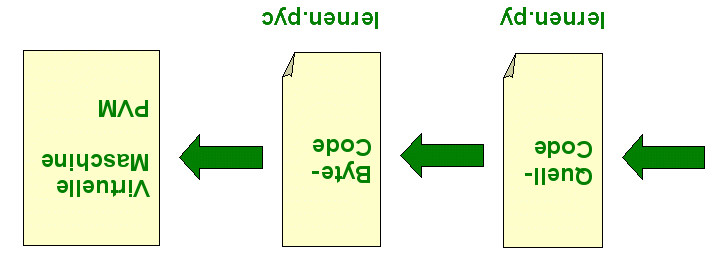
\includegraphics[width=0.7\linewidth]{pics/byte_code.png}
\label{fig:byte_code}
\end{minipage}
\\ \\ \\ \\
\\ \\ \\
\\ \\
\begin{MyConsoleBox}{
monty@python \$ python \\
Python 2.6.2 (release26-maint, Apr 19 2009, 01:58:18) \\
$[$GCC 4.3.3$]$ on linux2 \\
Type ''help'', ''copyright'', ''credits'' or ''license'' for more information. \\
${\Longrightarrow}$ import python\_lernen \\
Python lernen! \\
${\Longrightarrow}$ \\
monty@python \$ ls python\_lernen* \\
python\_lernen.py   python\_lernen.pyc \\
monty@python \$ 
}\end{MyConsoleBox}
\\
Bei einem späteren import in einem anderen Programmlauf, wird dann direkt die Datei mit dem Byte-Code geladen. Importiert man die gleiche Datei mehrmals im gleichen Skript wird sie nur beim ersten Mal geladen.\\
\\
Bei dem Byte-Code handelt es sich um einen Maschinenunabhängigen Code, der mittels einer virtuellen Maschine ausgeführt (PVM, Python Virtual Machine) wird. \\

\subsection{Compiler}
Ein Compiler (auch Übersetzer genannt) ist ein Computerprogramm, das ein in einer Quellsprache, wie beispielsweise C oder C++, geschriebenes Programm - Quelle oder Quellprogramm genannt - in ein semantisch äquivalentes Programm einer Zielsprache (Zielprogramm) übersetzt. Üblicherweise handelt es sich dabei um die Übersetzung eines von einem Programmierer in einer Programmiersprache geschriebenen Quelltextes in Assemblersprache, Bytecode oder Maschinensprache. Das Übersetzen eines Quellprogramms in ein Zielprogramm durch einen Compiler wird auch als Kompilierung bezeichnet. \\

\subsection{Interpreter}
Ein Interpreter ist ein Programm, das einen Quellcode im Gegensatz zu Assemblern oder Compilern nicht direkt in ausführbaren Code, also eine ausführbare Datei, wandelt, sondern den Quellcode einliest, analysiert und ausführt. Die Analyse des Quellcodes erfolgt zur Laufzeit des Programms. \\

\subsection{Strukturierung durch Einrückung}
Das Strukturierungsprinzip von Python unterscheidet sich deutlich von anderen Programmiersprachen. Andere Sprachen strukturieren (klammern) Programmblöcke durch Schlüsselwörter, wie beispielsweise ''begin'', ''end'', ''do'', ''done'' oder geschweiften Klammern. Leerzeichen, Folgen von Leerzeichen oder Einrückungen sind für die Compiler und Interpreter von den meisten Programmiersprachen ohne jede Semantik, d.h. sie werden überlesen. Dennoch wird Programmierern aber immer empfohlen, Blöcke durch gleichmäßgie Einrückungen für menschliche Benutzer kenntlich zu machen. In Python ist dies nun gänzlich anders. Hier haben Leerzeichen eine Bedeutung. Die Einrückung von Zeilen dient hier als Strukturierungselement, so dass Programmierer ''gezwungen'' werden übersichtlichen Code zu schreiben.\\
Ein häufiges Strukturierungselement sind Anweisungen die sich aus einem Anweisungskopf und einem Anweisungskörper zusammensetzen, wie z.B. die while- und die for-Schleife. \\

\begin{minipage}{-0.8\textwidth}
\centering
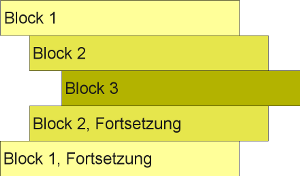
\includegraphics[width=5cm,height=2cm]{pics/bloecke300.png}
\label{fig:bloecke300}
\end{minipage}
\\
Wesentlich sind hierbei der Doppelpunkt am Ende des Anweisungskopfes und die gleichmäßige Einrückung der zugehörigen Anweisungen.

\subsection{Datentypen und Variablen}
Auch wenn man Variablen und Datentypen von anderen Programmiersprachen bereits zur Genüge zu kennen glaubt, sollte man dieses Kapitel dennoch zumindest überfliegen, denn einiges ist eben doch anders in Python. \\
\\
Eine Variable im allgemeinsten Sinne ist einfach ein Behälter (Container) zur Aufbewahrung von bestimmten Werten, also z.B. Strings oder Zahlen. Man kann im Verlauf des Programms auf diese Variablen, oder genauer auf den Wert ihres Inhaltes zugreifen, oder ihnen einen neuen Wert zuweisen.
In den meisten Programmiersprachen, wie z.B. C, ist es so, dass eine Variable einen festen Speicherplatz bezeichnet, in dem Werte eines bestimmten Datentyps abgelegt werden können. Während des Programmlaufes kann sich der Wert der Variable ändern, aber die Wertänderungen müssen vom gleichen Typ sein. Also man kann nicht in einer Variable zu einem bestimmten Zeitpunkt eine Integerzahl gespeichert haben und dann diesen Wert durch eine Fließkommazahl überschreiben. Ebenso ist der Speicherort der Variablen während des gesamten Laufes konstant, kann also nicht mehr geändert werden. In Sprachen wie C wird der Speicherort bereit durch den Compiler fixiert.
In Python sieht dies anders aus. Zunächst einmal bezeichnen Variablen in Python keinen bestimmten Typ und deshalb benötigt man auch in Python keine Typdeklaration. Benötigt man im Programm bespielsweise eine Variable i mit dem Wert 42, so erreicht man dies einfach mit der folgenden Anweisung: \\
\\
\begin{MyConsoleBox}{
i = 42
}\end{MyConsoleBox}
\\ \\
Obige Anweisung darf man nicht als mathematisches Gleichheitszeichen sehen, sondern als ''der Variablen \textbf{i} wird der Wert 42 zugewiesen'', d.h. der Inhalt von i ist nach der Zuweisung 42. Man kann diesen Wert der Variablen auch, wie man im folgenden Beispiel sieht, anschließend ändern:  \\
\\
\begin{MyConsoleBox}{
${\Longrightarrow}$ i = 42 \\
${\Longrightarrow}$ i = i + 1 \\
${\Longrightarrow}$ print i \\
43 \\
${\Longrightarrow}$ \\
}\end{MyConsoleBox}
\\
\subsection{Zahlen}
Python kennt vier eingebaute (built-in) Datentypen für Zahlen:\\
\begin{itemize}
\item Ganzzahl (Integer) z.B. 4321
vorangestellte 0 bedeutet Oktalzahl und
vorangestelltes 0x bedeutet Hexzahl
\item lange Ganzzahl
Sie können beliebig lang werden
Sie werden mit einem l am Anfang bzw. L am Ende bezeichnet.
\item Fließkommazahlen
Zahlen der Form 3.14159 oder 17.3e+02
\item komplexe Zahlen
z.B. 1.2+3j
\end{itemize}

\subsection{Zeichenketten - Strings}
Ein String, oder Zeichenkette, kann man als eine Sequenz von einzelnen Zeichen sehen.\\
\\
\begin{minipage}{-0.8\textwidth}
\centering
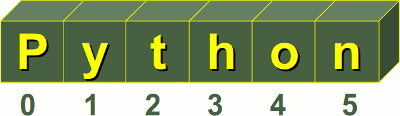
\includegraphics[width=4cm,height=1.2cm]{pics/string_indices.png}
\end{minipage}
\\ \\
Jedes einzelne Zeichen eines Strings, kann über einen Index angesprochen werden. Im folgenden Beispiel sehen wir, wie der obige im Bild dargestellt String in Python definiert wird und wie wir auf ihn zugreifen können: \\
\\
\begin{MyConsoleBox}{
${\Longrightarrow}$  s = ''Python'' \\
${\Longrightarrow}$  print s$[0]$ \\
P \\
${\Longrightarrow}$ print s$[3]$ \\
h \\
}\end{MyConsoleBox}\\
\\
Die Länge eines Strings kann man mit der Funktion len() bestimmen und damit kann man auch einfach beispielsweise auf das letzte oder vorletzte Zeichen eines Strings zugreifen: \\
\\
\begin{MyConsoleBox}{
${\Longrightarrow}$ s = ''Python'' \\
${\Longrightarrow}$ index\_last\_char = len(s) - 1 \\
${\Longrightarrow}$ print s$[$index\_last\_char$]$ \\
n \\
${\Longrightarrow}$ print s$[$index\_last\_char - 1$]$ \\
o \\
${\Longrightarrow}$ \\
}\end{MyConsoleBox} \\
\\
Der Indexzähler beginnt immer bei 0 an aufwärts zu zählen.\\
\\
Da es bei der praktischen Arbeit sehr häufig vorkommt, dass man auf einzelne Zeichen eines Strings von hinten zugreifen muss, wäre es sehr lästig, wenn man dies immer über den Umweg durch den Aufruf der Funktion len() machen müsste. Python bietet deshalb eine elegantere Möglichkeiten. Die Indices werden auch von rechts durch negative Indices nummeriert, d.h. das letzte Zeichen wird mittels des Index -1, das vorletzte mittels -2 usw. angesprochen. \\
\\
\begin{minipage}{-0.8\textwidth}
\centering
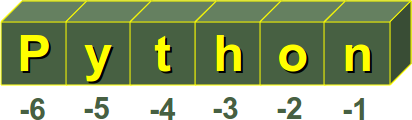
\includegraphics[width=4cm, height=1.2cm]{pics/string_indices_negative.png}
\label{fig:string_indices_negative}
\end{minipage} \\
\\
Strings können unter Benutzung von\\
\begin{itemize}
\item \textbf{Konkatenation/Verbinden} (englisch: Concatenation)\\
Diese Funktion dient dazu mittels des ''+''-Operators zwei Strings zu einem neuen String zusammenzuhängen:
''Hello'' + ''World'' $\Rightarrow$ ''HelloWorld''
\item \textbf{Wiederholung} (englisch: Repetition) \\
Ein String kann wiederholt konkateniert werden. Dazu benutzt man den '*'-Operator.
Beispiel:\\
''*-*'' * 3 wird zu ''*-**-**-*''
\item \textbf{Indexing} \\
''Python''[0] $\Rightarrow$ ''P''
\item \textbf{Slicing}\\
Das englische Verb ''to slice'' bedeutet in Deutsch ''schneiden'' oder auch ''in Scheiben schneiden''. Letztere Bedeutung entspricht auch der Funktion von Slicing in Python. Man schneidet sich gewissermaßen eine ''Scheibe'' aus einem String heraus. [2:4] bedeutet im folgenden Ausdruck, dass wir aus dem String ''Python'' einen Teilstring herausschneiden, der mit dem Zeichen des Index 2 (inklusive) beginnt und bis zum Index 4 (exklusive) geht: \\
\\
''Python''$[2:4]$ $\Rightarrow$ ''th'' \\
\\
\begin{minipage}{-0.8\textwidth}
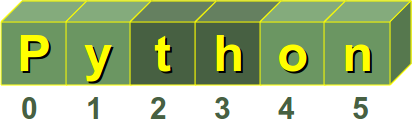
\includegraphics[width=4cm, height=1.2cm]{pics/string_slicing.png}
\label{fig:string_slicing}
\end{minipage}
\item \textbf{Länge} eines Strings \\
len(''Python'') $\Rightarrow$ 6 
\end{itemize}
angegeben werden. \\
\\
\subsection{Unveränderliche Zeichenketten}
Wie in Java aber nicht wie in C oder C++, können Strings in Python nicht verändert werden. Versucht man eine indizierte Position zu ändern, erzeugt man eine Fehlermeldung: \\
\\
\begin{MyConsoleBox}{
${\Longrightarrow}$ s = ''Some things are immutable!'' \\
${\Longrightarrow}$ s[-1] = ''.'' \\
Traceback (most recent call last): \\
\hspace{0.2cm} File ''$<$stdin$>$'', line 1, in $<$module$>$ \\
TypeError: 'str' object does not support item assignment \\
${\Longrightarrow}$ \\
}\end{MyConsoleBox}
\\

\subsection{Escape- oder Fluchtzeichen}
Es gibt Zeichenfolgen, die den Textfluss steuern, wie zum Beispiel ein Newline (Zeilenvorschub) oder Tabulator. Sie lassen sich nicht auf dem Bildschirm als einzelne Zeichen darstellen. Die Darstellung solcher Zeichen innerhalb von String-Literalen erfolgt mittels spezieller Zeichenfolgen, sogenannter Escape-Sequenzen. Eine Escape-Sequenz wird von einem Backslash \ eingeleitet, gefolgt von der Kennung des gewünschten Sonderzeichens. Übersicht der Escape-Zeichen:
\\
\begin{itemize}
\item $\setminus$ Zeilenfortsetzung 
\item $\setminus\setminus$ Rückwärtsschrägstrich 
\item $\setminus$' Einzelnes Anführungszeichen 
\item $\setminus$'' Doppeltes Anführungszeichen
\item $\setminus$a Glocke
\item $\setminus$b Rückschritt
\item $\setminus$e Ausmaskieren
\item $\setminus$0 Null
\item $\setminus$n Zeilenvorschub (linefeed, LF)
\item $\setminus$v Vertikaler Tabulator
\item $\setminus$t Horizontaler Tabulator
\item $\setminus$r Wagenrücklauf (carriage return, CR)
\item $\setminus$f Seitenvorschub
\item $\setminus$0XX Oktaler Wert
\item $\setminus$xXX Hexadezimaler Wert 
\end{itemize}
Die Auswertung von Escape-Zeichen kann man verhindern, indem man einem String ein r oder R unmittelbar voranstellt. \\
Beispiel: \\
r''$\setminus$n bewirkt einen Zeilenvorschub''

\subsection{Typwechsel bei Variablen}
In Python kann eine Variable, wie bereits gesagt, sofort ohne Deklaration des Datentyps verwendet werden. Dennoch vergibt Python einen Datentyp, d.h. je nach Datentyp, wird die Variable anders angelegt, also als Integer, Float, String, und so weiter. Eigentlich müsste man sagen, dass eine Objekt mit einem bestimmten Datentyp bzw. Klasse angelegt wird. Die Variable referenziert dann dieses Objekt, d.h. die Variable selbst hat also eigentlich keinen Typ. Anders ausgedrückt
Der Datentyp ist in Python nicht an die Variable, sondern an den Wert gebunden, was impliziert, dass sich der Typ zur Laufzeit ändern kann, wie wir im folgenden Beispiel sehen können:\\
\\
\begin{MyConsoleBox}{
i = 42         \hspace{1.5cm} \# Datentyp ist integer (implizit) \\
i = 42 + 0.11  \hspace{0.52cm}\# Typ ändert sich zu float \\
i = ''fourty'' \hspace{0.6cm} \# und jetzt ein String   \\
}\end{MyConsoleBox}
\\
\subsection{Wechselnde Speicherorte}
Prinzipiell wird sich im vorigen Fall, wobei das natürlich implementierungsabhängig ist, der Speicherort für die Variable i ändern. Der Interpreter kann bei der Anweisung ''i = 42'' den Wert als Integer abspeichern, muss aber bei der Anweisung ''i = 42 + 0.11'' einen neuen Ort für eine Float-Zahl anlegen. Für i = ''fourty'' muss er in einen String gewandelt werden.
Achtung: Als Anwender braucht man dies eigentlich nicht zu wissen, da ja alles automatisch geschieht! \\
\\
Betrachten wir nun folgenden Python-Code: \\
\\
\begin{MyConsoleBox}{
${\Longrightarrow}$ x = 3 \\
${\Longrightarrow}$ y = x \\
${\Longrightarrow}$ y = 2 \\
}\end{MyConsoleBox}
\\
Intuitiv würde man davon ausgehen, dass Python zunächst für x einen Speicherort wählt und dort das Objekt (Zahl) 3 abspeichert. Anschließend wird der Variablen y der Wert von x zugewiesen. In C und vielen anderen Programmiersprachen würde auch für y ein eigener Speicherort bestehen, in dem nun die Zahl 3 hineingeschrieben würde. Python geht anders vor: x ist eine Variable mit dem Objekt 3 und y ist eine Variable mit dem ''selben'' (nicht ''gleichen'') Objekt. x und y ''zeigen'' auf das gleiche Objekt. In der letzten Zeile wird y nun der Wert 2 zugewiesen, jetzt muss ein neues Objekt angelegt werden und y ''zeigt'' auf einen neuen Speicherort. (Anm: Dieses eben verwendete 'zeigen' sollte von C-Programmierern keinesfalls mit den unter C verwendeten Pointern verwechselt werden.)\\
\\
Es stellt sich nun die Frage, wie man das oben gesagte überprüfen kann. Dazu bietet sich die Identitätsfuntion id() an. Die Identität einer Instanz dient dazu, sie von allen anderen Instanzen zu unterscheiden. Die Identität ist eine Ganzzahl, und sie ist innerhalb eines Programmes eindeutig. Die Identitätsfunktion id() liefert die Identität. So kann man prüfen, ob es sich um eine bestimmte Instanz handelt und nicht nur um eine mit dem gleichen Wert und Typ. Wir geben nochmals das obige Beispiel ein, lassen uns aber jeweils die Identität ausgeben: \\
\\
\begin{MyConsoleBox}{
${\Longrightarrow}$ x = 3 \\
${\Longrightarrow}$ print id(x) \\
157379912 \\
${\Longrightarrow}$ y = x \\
${\Longrightarrow}$ print id(y) \\
157379912 \\
${\Longrightarrow}$ y = 2 \\
${\Longrightarrow}$ print id(y) \\
157379924 \\
${\Longrightarrow}$ print id(x) \\
157379912 \\
${\Longrightarrow}$ \\
}\end{MyConsoleBox}
\\ \\ \\
Wir stellen fest, dass sich die Identität erst ändert, nachdem wir y einen neuen Wert zugewiesen haben. Die Identität von x bleibt gleich, d.h. der Speicherort von x wird nicht geändert. \\
\\

\subsection{Besonderheiten bei Strings}
Einen besonderen Effekt können wir bei Strings feststellen. Im folgenden Beispiel wollen wir dies veranschaulichen. Dazu benötigen wir noch den 'is'-Operator. Sind a und b zwei Strings, dann prüft ''a is b'', ob a und b die gleiche Identität (Speicherort) haben. Wenn 'a is b' gilt, dann gilt auch ''a == b''. Aber wenn ''a == b'' gilt, dann gilt natürlich nicht notwendigerweise auch ''a is b''!
Nun wollen wir untersuchen, wie Strings in Python abgespeichert werden. Im folgenden Beispiel, erkennen wir, dass a und b sich den gleichen Speicherort teilen, obwohl wir diesmal keine Zuweisung der Art ''b = a'' verwendet haben: \\
\\
\begin{MyConsoleBox}{
${\Longrightarrow}$ a = ''Linux'' \\
${\Longrightarrow}$ b = ''Linux'' \\
${\Longrightarrow}$ a is b \\
True \\
\\
${\Longrightarrow}$ a = ''Baden-Württemberg'' \\
${\Longrightarrow}$ b = ''Baden-Württemberg'' \\
${\Longrightarrow}$ $a is b$ \\
False \\
${\Longrightarrow}$ $a == b$ \\
True \\
}\end{MyConsoleBox}
\\

\section{Ausdrücke und Operatoren}
Unter einem Ausdruck in Python und in anderen Programmiersprachen versteht man eine Kombination aus Variablen, Konstanten, Operatoren und Rückgabewerten von Funktionen. Die Auswertung eines Ausdrucks ergibt einen Wert, der meistens einer Variablen zugewiesen wird. In Python werden Ausdrücke unter Verwendung der gebräuchlichen mathematischen Notationen und Symbolen für Operatoren geschrieben. 

\subsection{Operatoren}
Die meisten Operatoren für Zahlenwerte sind in Python ähnlich zu anderen Programmiersprachen. Wir geben hier eine Übersicht, ohne sie vollständig zu erklären. Bei Bedarf werden diese Operatoren in anderen Kapitel besprochen. \\
\\
\begin{MyTableBox}{
\textbf{Operator}      & \textbf{Bezeichnung}               & \textbf{Beispiel}       \\ \hline
+, -                   & Addition, Subtraktion              & 10 -3                   \\ \hline
*, /, \%               & Multiplikation, Division, Rest     &                         \\ \hline
+x, -x                 & Vorzeichen                         & -3                      \\ \hline
\textasciitilde x      & Bitweises Not                      & \textasciitilde 3 - 4   \\ \hline
or, and, not           & Boolsches Oder, Und, Nicht         & (a or b) and c          \\ \hline
in                     & ''Element von''                    & 1 in [3, 2, 1]          \\ \hline
$<, <=, >, >=, !=, ==$ & Vergleichsoperatoren               & 2 $<=$ 3                \\ \hline
\textbar, \& , \textasciicircum & Bitweises Oder, Und, XOR  & 6 {\textasciicircum} 3  \\ \hline
$\ll, \gg$             &  Shiftoperatoren                   & 6 $\ll$ 2               \\
}\end{MyTableBox}
\\

\section{Tiefes und flaches Kopieren}
Wie wir im letzten Kapitel ''Datentypen und Variablen'' gesehen haben, verhält sich Python beim Kopieren einfacher Datentypen wie Integer und Strings ungewöhnlich im Vergleich zu anderen Programmiersprachen.
In dem folgenden Code-Beispiel zeigt y zunächst nur auf den gleichen Speicherplatz wie x. Erst wenn der Wert von y verändert wird, erhält y einen eigenen Speicherplatz, wie wir im vorigen Kapitel gesehen haben. \\
\\
\begin{MyConsoleBox}{
${\Longrightarrow}$ x = 3 \\
${\Longrightarrow}$ y = x \\
}\end{MyConsoleBox}
\\
Aber auch wenn das obige Verhalten ungewöhlich im Vergleich zu anderen Programmiersprachen wie C, C++, Perl und anderen ist, so entsprechen die Resultate der Zuweisungen dennoch unseren Erwartungen. Kritisch wird es jedoch, wenn wir mutable Objekte wie Listen und Dictionarys kopieren wollen. Python legt nur dann echte Kopien an, wenn es unbedingt muss, d.h. dass es der Anwender, also der Programmierer, explizit verlangt. In diesem Kapitel wollen wir einige Probleme aufzeigen, die beim Kopieren von mutablen Objekten entstehen können, also z.B. beim kopieren von Listen und Dictionaries. \\
\\
\subsection{Kopieren einer Liste}
\begin{MyConsoleBox}{
${\Longrightarrow}$ colours1 = $[$ ''red'', ''green'' $]$  \\
${\Longrightarrow}$ colours2 = colours1          \\
${\Longrightarrow}$ colours2 = $[$ ''rouge'', ''vert'' $]$ \\
${\Longrightarrow}$ print colours1               \\
$[$ 'red', 'green' $]$ \\
}\end{MyConsoleBox}
\\
In dem obigen Code-Beispiel legen wir zuerst eine einfache Liste colours1 an, die wir dann in colours2 kopieren. Anschließend weisen wir colours2 eine neue Liste zu.\\
\\
Es erstaunt wenig, dass die Werte von colours1 dabei unverändert bleiben. Wie bei dem Beispiel mit den Integer-Variablen im letzten Kapitel ''Datentypen und Variablen'' wird ein neuer Speicherbereich für colours2 angelegt, als dieser Variablen eine komplett neue Liste zugeordnet wird. \\
\\
\begin{MyConsoleBox}{
${\Longrightarrow}$ colours1 = [''red'', ''green''] \\
${\Longrightarrow}$ colours2 = colours1             \\
${\Longrightarrow}$ colours2$[1]$ = ''blue''        \\
${\Longrightarrow}$ colours1                    \\
$[$ 'red', 'blue' $]$  \\
}\end{MyConsoleBox}
\\
Wie sieht es jedoch aus, wenn nur einzelne Elemente geändert werden?
Um dies zu testen weisen wir dem zweiten Element von colours2 einen neuen Wert zu. Viele wird es nun erstauen, dass auch colours1 damit verändert wurde, obwohl man doch eine Kopie von colours1 gemacht zu haben glaubte. Die Erklärung ist, dass das zugehörige Objekt von colours2 nicht geändert wurde. \\
\\
Mit dem Teilbereichsoperator (slicing) kann man flache Listenstrukturen komplett kopieren, ohne dass es zu Seiteneffekten kommt, wie man im folgenden Beispiel sehen kann: \\
\\
\begin{MyConsoleBox}{
${\Longrightarrow}$ liste1 = $[$ 'a','b','c','d' $]$ \\
${\Longrightarrow}$ liste2 = liste1$[:]$           \\
${\Longrightarrow}$ liste2 $[1]$ = 'x'              \\
${\Longrightarrow}$ print liste2  \\
$[$ 'a', 'x', 'c', 'd' $]$ \\
${\Longrightarrow}$ print liste1 \\
$[$ 'a', 'b', 'c', 'd '$]$ \\
${\Longrightarrow}$
}\end{MyConsoleBox}
\\
Sobald jedoch auch Unterlisten in der zu kopierenden Liste vorkommen, werden nur Zeiger auf diese Unterlisten kopiert. \\
\\
\begin{MyConsoleBox}{
${\Longrightarrow}$ lst1 = $[$'a','b',$[$'ab','ba'$]]$ \\
${\Longrightarrow}$ lst2 = lst1$[:]$
}\end{MyConsoleBox}
\\
Weist man nun zum Beispiel dem 0-ten Element einer der beiden Listen einen neuen Wert zu, führt dies nicht zu einem Seiteneffekt. Probleme gibt es erst, wenn man direkt eines der beiden Elemente der Unterliste verändert.
Um dies zu demonstrieren, ändern wir nun zwei Einträge in lst2: \\
\\
\begin{MyConsoleBox}{
${\Longrightarrow}$ lst1 = $[$'a','b',$[$'ab','ba'$]]$ \\
${\Longrightarrow}$ lst2 = lst1$[$:$]$ \\
${\Longrightarrow}$ lst2$[0]$ = 'c' \\
${\Longrightarrow}$ lst2$[2][1]$ = 'd' \\
${\Longrightarrow}$ print(lst1) \\
$[$'a', 'b', $[$'ab', 'd'$]]$ \\
${\Longrightarrow}$
}\end{MyConsoleBox}
\\ \\
Man erkennt, dass man aber nicht nur die Einträge in lst2 geändert hat, sondern auch den Eintrag von lst1$[2][1]$.
Dies liegt daran, dass in beiden Listen, also lst1 und lst2, das jeweils dritte Element nur ein Link auf eine physikalisch gleiche Unterliste ist. Diese Unterliste wurde nicht mit $[:]$ mitkopiert. \\
\\
\subsection{Kopie mit der Methode deepcopy aus dem Modul copy}
Abhilfe für das eben beschriebene Problem schafft das Modul ''copy''. Dieses Modul stellt die Methode ''deepcopy'' zur Verfügung, die das komplette Kopieren einer nicht flachen Listenstruktur erlaubt.\\
Das folgende Skript kopiert unser obiges Beispiel nun mit Hilfe dieser Methode:\\
\\
\begin{MyConsoleBox}{
from copy import deepcopy \\
\\
lst1 = $[$'a','b',$[$'ab','ba'$]]$ \\
\\
lst2 = deepcopy(lst1) \\
\\
lst2$[2][1]$ = ''d'' \\
lst2$[0]$ = ''c''; \\
\\
print lst2 \\
print lst1 \\
}\end{MyConsoleBox}
\\ \\
Speichern wir das Skript unter deep\_copy.py ab und rufen es mit ''python deep\_copy.py'' auf, so erhalten wir folgende Ausgabe: \\
\begin{MyConsoleBox}{
\$ python deep\_copy.py 
$[$'c', 'b', $[$'ab', 'd'$]]$ \\
$[$'a', 'b', $[$'ab', 'ba'$]]$
}\end{MyConsoleBox}
\\
\section{Bedingte Anweisungen}
Zu bestimmten Zeiten sind gewisse Entscheidungen unvermeidlich, wie man im Foto sehen kann. So kann man kaum ein sinnvolles Programm schreiben, welches ohne jede Verzweigung auskommt. Bisher sind wir in der Lage Programme zu schreiben, in denen eine Anweisung auf die andere folgt und diese auch in dieser Reihenfolge ausgeführt werden. Aber nur wenige Probleme lassen sich durch einen linearen Programmablauf kontrollieren. Man möchte beispielsweise einen bestimmten Teil des Programmes nur dann ausführen, wenn bestimmte Bedingungen zutreffen oder ein anderer Teil soll gegebenenfalls mehrmals ausgeführt werden. Dazu bietet jede Programmiersprache Kontrollstrukturen, die sich in zwei Kategorien unterscheiden lassen: Verzweigungen und Schleifen.\\
\\
In einer Programmiersprache versteht man unter einer bedingten Anweisung, wie man Verzweigungen auch nennt, Codeteile, die unter bestimmten Bedingungen ausgeführt werden. Liegt die Bedingung nicht vor, wird dieser Code nicht ausgeführt. Anders ausgedrückt: Eine Verzweigung legt fest welcher von zwei (oder auch mehr) Programmteilen (Alternativen) in Abhängigkeit von einer (oder mehreren) Bedingungen ausgeführt wird. Bedingte Anweisungen und Verzweigungen werden in Programmiersprachen (ebenso wie die Schleifen) den Kontrollstrukturen zugerechnet, weil mit ihrer Hilfe ein Programm auf verschiedene Zustände, die sich aus Eingaben und Berechnungen ergeben, reagieren kann.\\
\\
In dem abschließenden Beispiel dieses Kapitels geht es um Steuern. Wir schreiben ein Pythonskript, mit dem man sich aus dem zu versteuernden Einkommen die Steuern für 2010 berechnen lassen kann. 
\\
\subsection{Die if-Anweisung}
Die allgemeine Form der if-Anweisung sieht in Python wie folgt aus: \\
\\
\begin{MyConsoleBox}{
if bedingung1: \\
    anweisungen1 \\
elif bedindung2: \\
    anweisungen2 \\
else: \\
    anweisungen3 \\
}\end{MyConsoleBox}
\\ \\
Falls die Bedingung ''bedingung1'' wahr ist, werden die Anweisungen ''anweisungen1'' ausgeführt. Wenn nicht, werden, falls bedingung2 wahr ist, die anweisungen2 ausgeführt. Falls weder die erste Bedingung (bedingung1) noch die zweite Bedingung (bedingung2) wahr ist, werden die Anweisungen nach dem else (anweisungen3) ausgeführt. 
\\
\subsection{Beispiel Hundejahre}
Kinder und Hundeliebhaber stellen sich häufig die Frage, wie alt ihr Hund wohl wäre, wenn er kein Hund sondern ein Mensch wäre. Landläufig rechnet man Hundejahre in Menschjahre um, indem man das Alter des Hundes mit 7 multipliziert. Je nach Hundegröße und Rasse sieht die Umrechnung jedoch etwas komplizierter aus, z.B.: 
\\
\begin{MyConsoleBox}{
age = input(''Alter des Hundes: '')     \\
print                                   \\
if age $<$ 0:                           \\
	print ''Das stimmt wohl kaum!''     \\
elif age $==$ 1:                          \\
	print ''entspricht ca. 14 Jahre''   \\
elif age $==$ 2:                          \\
	print ''entspricht ca. 22 Jahre''   \\
elif age $>$ 2:                         \\
	human = 22 + (age -2)*5             \\
	print ''Menschenjahre', human       \\
                                        \\
\#\#\#                                  \\
raw\_input('press Return$>$')              \\
}\end{MyConsoleBox}
\\
\subsection{Wahr oder falsch}
Leider ist es nicht in allen Dingen des Lebens so einfach zwischen Wahr und Falsch zu unterscheiden wie in Python:
Als ''falsch'' gelten \\
\\
\begin{itemize}
\item numerische Null-Werte(0, 0L, 0.0, 0.0+0.0j), 
\item der boolschen Wert False, 
\item leere Zeichenketten, 
\item leere Listen, leere Tupel, 
\item leere Dictionaries. 
\item sowie der spezielle Wert None. 
\end{itemize}
Alle anderen Werte betrachtet Python als ''wahr''.
\\
\subsection{Abgekürztes IF}
C-Programmierer kennen folgende abgekürzte Schreibweise für das if-Konstrukt: \\
\begin{MyConsoleBox}{
max = (a $>$ b) ? a : b; 
}\end{MyConsoleBox}
\\
\\
als Abkürzung für: \\
\\
\begin{MyConsoleBox}{
if (a $>$ b) \\
   max=a;  \\
else       \\
   max=b;  \\
}\end{MyConsoleBox}
\\
\\
In Python müssen sich C-Programmierer, was diese Schreibweise betriff, umgewöhnen. In Python formuliert man das vorige Beispiel wie folgt:\\
\\
\begin{MyConsoleBox}{
max = a if (a $>$ b) else b;
}\end{MyConsoleBox}
\\
\subsection{Steuerrechner in Python}
Das zu versteuernde Einkommen (zvE) wird zunächst einer Tarifzone zugeordnet. Dann lässt sich der Steuerbetrag (StB) bei Einzelveranlagung nach der entsprechenden Formel berechnen.\\
\\
\begin{itemize}
\item Erste Zone (Grundfreibetrag): bis 8004,- \EUR{} fällt keine Steuer an 
\item Zweite Zone: zvE von 8.005 \EUR{} bis 13.469 \EUR{} \\
StB = (912,17 * y + 1400)*y \\
Für y gilt: \\
y = (zvE - 8004) / 10000 
\item Dritte Zone: zvE von 13470 \EUR{} bis 52881 \EUR{} \\
StB = (228,74 * z + 2397)*z \\
Für z gilt: \\
z = (zvE - 13469) / 10000
\item Vierte Zone: zvE von 52882 \EUR{} bis 250730 \EUR{} \\
StB = 0,42 * zvE - 8172 
\item Fünfte Zone: zvE ab 250731 \EUR{} \\
StB = 0,44 * zvE - 15694 
\end{itemize}
Eine Python-Funktion zur Berechnung der Steuer aus dem Einkommentarif sieht nun wie folgt aus: (natürlich ohne Gewähr!!!) \\
\\
\begin{MyConsoleBox}{
def steuern(einkommen):\\
\hspace{0.5cm}    ''''''Berechnung der zu zahlenden Steuern fuer ein zu versteuerndes Einkommen von x'''''' \\
\hspace{0.5cm}    if einkommen $<=$ 8004: \\
\hspace{1.0cm}         steuer = 0 \\
\hspace{0.5cm}    elif einkommen $<=$ 13469: \\
\hspace{1.0cm}         y = (einkommen -8004.0)/10000.0 \\
\hspace{1.0cm}         steuer = (912.17 * y + 1400)*y \\
\hspace{0.5cm}    elif einkommen $<=$ 52881: \\
\hspace{1.0cm}         z = (einkommen -13469.0)/10000.0 \\
\hspace{1.0cm}         steuer = (228.74 * z +2397.0)*z +1038.0 \\
\hspace{0.5cm}    elif einkommen $<=$ 250730: \\
\hspace{1.0cm}         steuer = einkommen * 0.42 - 8172.0 \\
\hspace{0.5cm}    else: \\
\hspace{1.0cm}        steuer = einkommen * 0.44 - 15694 \\
\hspace{0.5cm}    return steuer \\
}\end{MyConsoleBox}

\section{Eingabe mit input()}
Es gibt kaum Programme, die ohne jegliche Eingaben auskommen. Eingaben können über viele Wege erfolgen, so zum Beispiel aus einer Datenbank, von einem anderen Rechner im lokalen Netzwerk oder auch über das Internet. Die einfachst und wohl auch häufigste Eingabe erfolgt jedoch über die Tastatur. Für diese Form der Eingabe bietet Python die Funktion input(text). \\
\\
Kommt es zum Aufruf der Funktion input während eines Programmlaufes, wird der Programmablauf solange gestoppt, bis die Benutzerin oder der Benutzer eine Eingabe über die Tastur tätigt und diese mit der Return-Taste abschließt. Damit der User auch weiß, was er einzugeben hat, wird der String des Parameters "text" ausgegeben, sofern ein solcher String existiert. Der Parameter von input() ist optional. \\
\\
Der Eingabestring des Benutzers wird von input() interpretiert, d.h. input() liefert beispielsweise einen Integer Wert zurück, wenn der Benutzer eine ganze Zahl eingeben hat und eine Liste, wenn der Benutzer eine Liste eingegeben hat. \\
\\
Wir zeigen dies in der folgenden interaktiven Python-Shell-Sitzung: \\
\\
\begin{MyConsoleBox}{
${\Longrightarrow}$ x = input(''Ihr Name? '') \\
Ihr Name? ''John'' \\
${\Longrightarrow}$ print(x) \\
John \\
${\Longrightarrow}$ x = input(''Ihre Gehalt? '') \\
Ihre Gehalt? 2877.03 \\
${\Longrightarrow}$ x \\
2877.03 \\
${\Longrightarrow}$ type(x) \\
$<$type 'float'$>$  \\
${\Longrightarrow}$ x = input(''Ihre Lieblingssprachen? '') \\
Ihre Lieblingssprachen? $[$ ''Java'', ''Perl'', ''C++'' $]$ \\
${\Longrightarrow}$ print(x) \\
$[$'Java', 'Perl', 'C++'$]$ \\
${\Longrightarrow}$ type(x) \\
$<$type 'list'$>$ \\
${\Longrightarrow}$ \\
}\end{MyConsoleBox}
\\
\section{Eingabe mit raw\_input()}
Anders als bei input, interpretiert raw\_input nicht die Eingabe. Das heißt, raw\_input liefert immer einen String zurück, d.h. der Eingabestring des Bentuzers wird unverändert weitergeleitet. Will man einen bestimmten Datentyp, so kann man die Eingabe durch die entsprechende Casting-Funktion wandeln oder man kann die eval-Funktion verwenden. Wir demonstrieren dies wieder an einigen Beispielen in der interaktiven Python-Shell: \\
\\
\begin{MyConsoleBox}{
${\Longrightarrow}$ x = raw\_input(''Ihr Name? '') \\
Ihr Name? John \\
${\Longrightarrow}$ print(x) \\
John \\
${\Longrightarrow}$ x = raw\_input(''Ihre Gehalt? '') \\
Ihre Gehalt? 2877.03 \\
${\Longrightarrow}$ print(x) \\
2877.03 \\
${\Longrightarrow}$ type(x) \\
$<$type 'str'$>$ \\
${\Longrightarrow}$ x = float(raw\_input(''Ihre Gehalt? '')) \\
Ihre Gehalt? 2877.03 \\
${\Longrightarrow}$ type(x) \\
$<$type 'float'$>$ \\
${\Longrightarrow}$ x = eval$($raw\_input$($''Ihre Lieblingssprachen? ''$))$ \\
Ihre Lieblingssprachen?  $[$''Java'', ''Perl'', ''C++''$]$ \\
${\Longrightarrow}$ print(x) \\
$[$'Java', 'Perl', 'C++'$]$ \\
${\Longrightarrow}$ type(x) \\
$<$type 'list'$>$ \\
${\Longrightarrow}$ \\
}\end{MyConsoleBox}

\section{Schleifen}
Schleifen, werden benötigt, um einen Codeblock, den man auch als Schleifenkörper bezeichnet, wiederholt auszuführen. In Python gibt es zwei Schleifentypen: die while-Schleife und die for-Schleife. \\
Die meisten Schleifen enthalten einen Zähler oder ganz allgemein Variablen, die im Verlauf der Berechnungen innerhalb des Schleifenkörpers ihre Werte ändern. Außerhalb, d.h. noch vor dem Beginn der Schleife, werden diese Variablen initialisiert. Vor jedem Schleifendurchlauf wird geprüft, ob ein Ausdruck, in dem diese Variable oder Variablen vorkommen, wahr ist. Dieser Ausdruck bestimmt das Endekriterium der Schleife. Solange die Berechnung dieses Ausdrucks "True" liefert wird der Rumpf der Schleife ausgeführt. Nachdem alle Anweisungen des Schleifenkörpers durchgeführt worden sind, springt die Programmsteuerung automatisch zum Anfang der Schleife, also zur Prüfung des Endekriteriums zurück und prüft wieder, ob diese nochmals erfüllt ist.
Wenn ja, geht es wie oben beschrieben weiter, ansonsten wird der Schleifenkörper nicht mehr ausgeführt und es wird mit dem Rest des Skriptes fortgefahren. Das nebenstehende Diagramm zeigt dies schematisch. \\
\\
Wir möchten dies nun an einem kleinen Python-Skript verdeutlichen, welches die Summe der Zahlen von 1 bis 100 bildet. Im nächsten Kapitel über for-Schleifen werden wir eine weitaus elegantere Möglichkeiten zu diesem Zweck kennenlernen. \\
\\
\begin{MyConsoleBox}{
n = 100 \\
\\
s = 0 \\
i = 1 \\
while i $<=$ n: \\
\hspace{0.5cm}    s = s + i \\
\hspace{0.5cm}    i = i + 1 \\
\\
print ''Die Summe lautet: '', s \\
}\end{MyConsoleBox}
\\
\subsection{Standard-Eingabe lesen}
Bevor wir mit der while-Schleife weitermachen, müssen wir noch ein paar grundsätzliche Dinge über die Standardeingabe und die Standardausgabe klären. Als Standardeingabe gilt normalerweise die Tastatur. Die meisten Shell-Programme schreiben ihre Ausgaben in die Standardausgabe, d.h. das Terminalfenster oder die Textkonsole. Fehlermeldungen werden in die Standard-Fehlerausgabe ausgegeben, was üblicherweise auch dem aktuellen Terminalfenster oder der Textkonsole entspricht.
Auch der Python-Interpreter stellt drei Standard-Dateiobjekte zur Verfügung: \\
\\
\begin{itemize}
\item Standardeingabe 
\item Standardausgabe 
\item Standardfehlerausgabe 
\end{itemize}
Sie stehen im Modul ''sys'' als: \\
\begin{itemize}
\item sys.stdin
\item sys.stdout
\item sys.stderr
\end{itemize}
zur Verfügung.\\
\\
Das folgende Beispiel-Skript zeigt nun, wie man Zeichen für Zeichen mittels einer while-Schleife von der Standardeingabe (Tastatur) einliest. Mit dem import-Befehl wird das benötigte Modul sys eingelesen. \\
\\
\begin{MyConsoleBox}{
import sys \\
\\
text = '''' \\
while 1: \\
\hspace{0.5cm}   c = sys.stdin.read(1) \\
\hspace{0.5cm}   text = text + c \\
\hspace{0.5cm}   if c == '$\setminus$n': \\
\hspace{1.0cm}       break \\
\\
print ''Eingabe: \%s'' \% text \\
}\end{MyConsoleBox}
\\
\\
Eleganter kann man eine beliebige Eingabezeile von der Standardeingabe natürlich mit der Funktion raw\_input(prompt) einlesen. \\
\\
\begin{MyConsoleBox}{
${\Longrightarrow}$ name = raw\_input(''Wie heißen Sie?$setminus$n'') \\
Wie heißen Sie? \\
Tux \\
${\Longrightarrow}$ print name \\
Tux \\
${\Longrightarrow}$ \\
}\end{MyConsoleBox}
\\
\subsection{Der else-Teil}
Wie auch die bedingte if-Anweisung hat die while-Schleife in Python im Gegensatz zu anderen Programmiersprachen einen optionalen else-Zweig, was für viele Programmierer gewöhnungsbedürftig ist.
Die Anweisungen im else-Teil werden ausgeführt, sobald die Bedingung nicht mehr erfüllt ist. Sicherlich fragen sich einige nun, worin dann der Unterschied zu einer normalen while-Schleife liegt. Hätte man die Anweisungen nicht in den else-Teil gesteckt sondern einfach hinter die while-Schleife gestellt, wären sie ja auch genauso ausgeführt worden. Es wird erst mit einem break-Kommando, was wir später kennenlernen sinnvoll.
Allgemein sieht eine while-Schleife mit else-Teil in Python wie folgt aus: \\
\\
\begin{MyConsoleBox}{
while Bedingung:          \\
\hspace{0.5cm} Anweisung1 \\
\hspace{0.5cm} \dots      \\
\hspace{0.5cm} Anweisungn \\
else:                     \\
\hspace{0.5cm} Anweisung1 \\
\hspace{0.5cm} \dots      \\
\hspace{0.5cm} Anweisungn \\
}\end{MyConsoleBox}

\subsection{Vorzeitiger Abbruch einer while-Schleife}
Normalerweise wird eine Schleife nur beendet, wenn die Bedingung im Schleifenkopf nicht mehr erfüllt ist. Mit break kann man aber eine Schleife vorzeitig verlassen und mit continue einen Durchlauf beenden.
Im folgenden Beispiel, einem einfachen Zahlenratespiel, kann mam erkennen, dass in Kombination mit einem break der else-Zweig durchaus sinnvoll sein kann. Nur wenn die while-Schleife regulär beendet wird, d.h. der Spieler die Zahl erraten hat, gibt es einen Glückwunsch. Gibt der Spieler auf, d.h. break, dann wird der else-Zweig der while-Schleife nicht ausgeführt. \\
\\
\begin{MyConsoleBox}{
import random												\\
n = 20														\\
to\_be\_guessed = int(n * random.random()) + 1				\\
guess = 0													\\
while guess $!=$ to\_be\_guessed:							\\
\hspace{0.5cm}    guess = input(''Neue Zahl: '')			\\
\hspace{0.5cm}    if guess $>$ 0:							\\
\hspace{1.0cm}        if guess $>$ to\_be\_guessed:			\\
\hspace{1.5cm}            print ''Zahl zu groß''			\\
\hspace{1.0cm}        elif guess $<$ to\_be\_guessed:		\\
\hspace{1.5cm}            print ''Zahl zu klein''			\\
\hspace{0.5cm}    else:										\\
\hspace{1.0cm}        print ''Schade, Sie geben also auf!'' \\
\hspace{1.0cm}        break									\\
else:														\\
\hspace{0.5cm}    print ''Glückwunsch! Das war's!'' 		\\
}\end{MyConsoleBox}
\\
\section{for-Schleifen}
Syntax:\\
\begin{MyConsoleBox}{
for Variable in Sequenz:		\\
\hspace{0.5cm}	Anweisung1		\\
\hspace{0.5cm}	Anweisung2		\\
\hspace{0.5cm}	\dots			\\
\hspace{0.5cm}	Anweisungn		\\
else:							\\
\hspace{0.5cm}	Else-Anweisung1 \\
\hspace{0.5cm}	Else-Anweisung2 \\
\hspace{0.5cm}	\dots			\\
\hspace{0.5cm}	Else-Anweisungm \\
}\end{MyConsoleBox}
\\
Die for-Anweisung hat einen unterschiedlichen Charakter zu den for-Schleifen, die man aus den meisten anderen Programmiersprachen kennt. In Python dient die for-Schleife zur Iteration über ein Sequenz von Objekten, während sie in anderen Sprachen meist nur "eine etwas andere while-Schleife" ist. \\
Beispiel einer for-Schleife in Python:  \\
\begin{MyConsoleBox}{
${\Longrightarrow}$ languages = [''C'', ''C++'', ''Perl'', ''Python''] \\
${\Longrightarrow}$ for x in languages: \\
\dots\hspace{0.5cm}     print x \\
\dots \\
C \\
C++ \\
Perl \\
Python \\
${\Longrightarrow}$  \\
}\end{MyConsoleBox}
\\
\section{Die range()-Funktion}
Mit Hilfe der range()-Funktion lässt sich die for-Schleife ideal für Iterationen nutzen. range() liefert Listen, die arithmetischen Aufzählungen entsprechen.
Beispiel: \\
\\
\begin{MyConsoleBox}{
${\Longrightarrow}$ range(10) \\
$[0, 1, 2, 3, 4, 5, 6, 7, 8, 9]$ \\
}\end{MyConsoleBox}
\\
Obiges Beispiel zeigt, dass Range mit einem Argument aufgerufen die Liste der Zahlen von 0 bis zu diesem Argument liefert.
range() kann aber auch mit zwei Argumenten aufgerufen werden: \\
\\
\begin{MyConsoleBox}{
range(begin, end)
}\end{MyConsoleBox}
\\
Dann wird eine Liste aller ganzen Zahlen von begin (einschließlich) bis end (aussschließlich) geliefert.
Als drittes Argument kann man range() noch die Schrittweite mitgeben.
Beispiel: \\
\\
\begin{MyConsoleBox}{
${\Longrightarrow}$ range(4,10) \\
$[4, 5, 6, 7, 8, 9]$ \\
${\Longrightarrow}$ range(4,50,5) \\
$[4, 9, 14, 19, 24, 29, 34, 39, 44, 49]$ \\
}\end{MyConsoleBox}
\\
Besonders sinnvoll wird die range()-Funktion im Zusammenspiel mit der for-Schleife. Im nachfolgenden Beispiel bilden wir die Summe der Zahlen von 1 bis 100: \\
\\
\begin{MyConsoleBox}{
n = 100 \\
s = 0 \\
for i in range(1, n+1): \\
\space{0.5cm}   s = s + i \\
print s \\
}\end{MyConsoleBox}
\\
In obigem kleinen Programm verbirgt sich aber noch ein schreckliches Effizienzproblem. Was geschieht bevor die for-Schleife ausgeführt wird? Python wertet zuerst den Aufruf range(1, n+1) aus. Das bedeutet, dass eine Liste mit 100 Zahlen erzeugt wird, also [1, 2, 3, 4, \dots 100]. Es werden zwar alle Zahlen dieser Liste innerhalb der Schleife benötigt, aber zu keinem Zeitpunkt die ganze Liste. Im vorigen Kapitel hatte wir dieses Problem mit einer while-Schleife gelöst und dort benötigten wir auch keine Liste. Python bietet eine Lösung für dieses Problem, indem es die Funktion xrange zur Verfügung stellt. xrange erzeugt ein iterierbares Objekt (iterable), das bedeutet, dass keine Liste erzeugt wird sondern zum Beispiel in einer for-Schleife über die Werte iteriert werden kann ohne dass die Liste erzeugt wird: \\
\\
\begin{MyConsoleBox}{
${\Longrightarrow}$ for i in xrange(1, 7): \\
\dots \hspace{0.5cm}     print(i) \\
\dots \hspace{0.5cm} \\
1 \\
2 \\
3 \\
4 \\
5 \\
6 \\
${\Longrightarrow}$ \\
}\end{MyConsoleBox}
\\
Obige Schleife verhält sich im Hinblick auf die Effizienz ähnlich wie folgende while-Schleife: \\
\\
\begin{MyConsoleBox}{
${\Longrightarrow}$ i = 1 \\
${\Longrightarrow}$ while i $<$ 7: \\
\dots\hspace{0.5cm}     print(i) \\
\dots\hspace{0.5cm}     i += 1 \\
\dots\hspace{0.5cm} \\
1 \\
2 \\
3 \\
4 \\
5 \\
6 \\
${\Longrightarrow}$ \\
}\end{MyConsoleBox}
\\
Im Ausgabeverhalten sieht man natürlich keinen Unterschied. Den Unterschied zwischen range und xrange sieht man aber, wenn man die Aufrufe direkt in der interaktiven Python-Shell tätigt: \\
\begin{MyConsoleBox}{
${\Longrightarrow}$ range(1,7)	\\
$[1, 2, 3, 4, 5, 6]$			\\
${\Longrightarrow}$ xrange(1,7) \\
xrange(1, 7)					\\
${\Longrightarrow}$
}\end{MyConsoleBox}
\\
Die meisten glauben, dass der Satz von Pythagoras von Pythagoras entdeckt worden war. Warum sonst sollte der Satz seinen Namen erhalten haben. Aber es gibt eine Debatte, ob dieser Satz nicht auch unabhängig von Pyhtagoras und vor allen Dingen bereits früher entdeckt worden sein könnte. Für die Pythagoräer - eine mystische Bewegung, die sich auf die Mathematik, Religion und die Philosophie begründete - waren die ganzen Zahlen, die den Satz des Pythagoras erfüllten besondere Zahlen, die für sie heilig waren.
\\
\\
\begin{figure}[h]
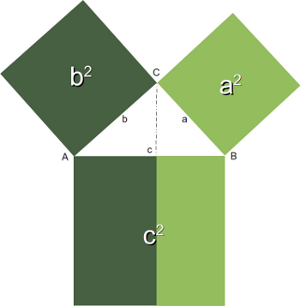
\includegraphics[width=4cm,height=4.5cm]{pics/pythagoras_beweis.png}
\caption[Pythagoras-Satz]{Pythagoras-Satz-Beweis}
\label{fig:pythagoras_beweis}
\end{figure}
\\
Heutzutage haben die Pythagoräischen Zahlen nichts mystisches mehr. Obwohl sie für manche Schülerin oder Schüler oder ander Personen, die mit der Mathematik auf Kriegsfuß stehen, immer noch so erscheinen mögen.
Ganz unromantisch gilt in der Mathematik:\\
Drei natürliche Zahlen, welche die Gleichung $a^2 + b^2 = c^2$ erfüllen, heißen pythagoräische Zahlen.
Das folgende Programm berechnet alle pythagoräischen Zahlen bis zu einer einzugebenden maximalen Zahl: \\
\\
\begin{MyConsoleBox}{
\#!/usr/bin/env python \\
from math import sqrt \\
n = raw\_input(''Maximale Zahl? '') \\
n = int(n)+1 \\
for a in xrange(1, n): \\
\hspace{0.5cm}    for b in xrange(a, n): \\
\hspace{1.0cm}        c\_square = a**2 + b**2 \\
\hspace{1.0cm}        c = int(sqrt(c\_square)) \\
\hspace{1.0cm}        if ((c\_square - c**2) == 0): \\
\hspace{1.5cm}            print a, b, c \\
}\end{MyConsoleBox}
\\
\section{Iteration über Liste mit range()}
Falls man auf die Indexe einer Liste zugreifen möchte, scheint es keine gute Idee zu sein eine For-Schleife zur Iteration über die Liste zu nutzen. Man kann dann zwar alle Elemente erreichen, aber der Index eines Elementes ist nicht verfügbar. Aber es gibt eine Möglichkeit sowohl auf den Index als auch auf das Element zugreifen zu können. Die Lösung besteht darin range() in Kombination mit der len()-Funktion, die einem die Anzahl der Listenelemente liefert, zu benutzen: \\
\\
\begin{MyConsoleBox}{
fibonacci = $[0,1,1,2,3,5,8,13,21]$ \\
for i in xrange(len(fibonacci)): \\
\hspace{0.5cm}    print i,fibonacci[i] \\
print \\
}\end{MyConsoleBox}
\\
\section{
Listen-Iteration mit Seiteneffekten}
Falls man über eine Liste iteriert, sollte man vermeiden die Liste im Schleifenkörper (body) zu verändern. Was passieren kann, zeigen wir im folgenden Beispiel: \\
\\
\begin{MyConsoleBox}{
colours = [''red''] \\
for i in colours: \\
\hspace{0.5cm}    if i == ''red'': \\
\hspace{1.0cm}        colours += [''black''] \\
\hspace{0.5cm}    if i == ''black'': \\
\hspace{1.0cm}        colours += [''white''] \\
print colours \\
}\end{MyConsoleBox}
\\
Was wird durch die Anweisung "print colours" ausgegeben? \\
\\
\begin{MyConsoleBox}{
['red', 'black', 'white']
}\end{MyConsoleBox}
\\
Am besten benutzt man eine Kopie der Liste, wie im nächsten Beispiel: \\
\\
\begin{MyConsoleBox}{
colours = [''red''] \\
for i in colours[:]: \\
\hspace{0.5cm}    if i == ''red'': \\
\hspace{1.0cm}        colours += [''black''] \\
\hspace{0.5cm}    if i == ''black'': \\
\hspace{1.0cm}        colours += [''white''] \\
print colours \\
}\end{MyConsoleBox}
\\
Die Ausgabe sieht nun wie folgt aus: \\
\\
\begin{MyConsoleBox}{
['red', 'black']
}\end{MyConsoleBox}
\\
Auch jetzt haben wir die Liste verändert, aber ''bewusst'' innerhalb des Schleifenkörpers. Aber der Elemente, die über die For-Schleife interiert werden, bleiben unverändert durch die Iterationen. \\
\\
\section{Ausgabe mit print}
Es gibt eigentlich keine Computer-Programme und natürlich auch keine Python-Programme, die nicht in irgendeiner Weise mit der Außenwelt kommunizieren. Vor allen Dingen muss ein Programm immer Ergebnisse ausgeben. Eine Form der Ausgabe von Ergebnisse geht direkt in die Standardausgabe und dies erfolgt in Python mittels der print-Anweisung.\\
\\
\begin{MyConsoleBox}{
${\Longrightarrow}$ print ''Hallo Benutzer'' \\
Hallo Benutzer \\
${\Longrightarrow}$ antwort = 42 \\
${\Longrightarrow}$ print ''Die Antwort lautet: '' + str(antwort) \\
Die Antwort lautet: 42 \\
${\Longrightarrow}$ \\
}\end{MyConsoleBox}
\\
Ab Python3 ist print keine Anweisung mehr, sondern eine Funktion. Deshalb müssen die Argumente in Klammern geschrieben werden. Auch in Python2 kann man print mit Klammern schreiben:\\
\\
\begin{MyConsoleBox}{
${\Longrightarrow}$ print(''Hallo'') \\
Hallo \\
${\Longrightarrow}$ print(''Hallo'',''Python'') \\
('Hallo', 'Python') \\
${\Longrightarrow}$ print ''Hallo'',''Python'' \\
Hallo Python \\
${\Longrightarrow}$ \\ 
}\end{MyConsoleBox}
\\
Wir können erkennen, dass es dann ein geändertes Ausgabeverhalten gibt. Aber was noch schwerwiegender ist. Das Ausgabeverhalten mit runden Klammern in Python 2.x ist auch anders als das der Python-Funktion von Version 3.x, wie wir im Folgenden sehen können: \\
\\
\begin{MyConsoleBox}{
\$ python3 \\
Python 3.2.3 (default, Apr 10 2013, 05:03:36)  \\
$[$GCC 4.7.2$]$ on linux2 \\
Type ''help'', ''copyright'', ''credits'' or ''license'' for more information. \\
${\Longrightarrow}$ print(''Hallo'') \\
Hallo \\
${\Longrightarrow}$ print(''Hallo'',''Python'') \\
Hallo Python \\
${\Longrightarrow}$  \\
}\end{MyConsoleBox}
\\
\subsection{Import aus der Zukunft: print\_function}
In manchen Python2-Programmen findet sich die folgende Import-Zeile: \\
\\
\begin{MyConsoleBox}{
from \_\_future\_\_ import print\_function
}\end{MyConsoleBox}
\\
Dies ist auf den ersten Blick missverständlich. Es sieht so aus, als habe man eine Funktion namens ''print\_function'' importiert. Es wurde aber nur ein Flag, eine Instanz ''print\_function'' gesetzt. Dadurch wird in Python2 die print-Funktion von Python3 eingeführt. Das bedeutet, dass dann der Interpreter nur noch die Python3-Syntax der Print-Funktion akzeptiert. Das Programm verhält sich damit, zumindest was die print-Funktion betrifft, kompatibel zu Python3.\\
\\
Wenn Sie Programme in Python 2.6 oder Python 2.7 erstellen wollen, empfehlen wir Ihnen, diese immer mit obigem Import zu versehen. Dadurch ist sichergestellt, dass Ihre Ausgaben kompatibel zu Python 3 sind. \\
\\
\chapter{Grundlagen - Mathematik}\label{Mathegrundlagen}
\section{Zahlensysteme}\label{Zahlensysteme}
In jedem Zahlensystem wird der Wert einer Ziffer durch ihre Stellung
innerhalb einer Zahl bestimmt. Die Grundlage eines jedem Zahlensystems ist
seine Basis.
\\
\begin{minipage}{1.5\textwidth}
\begin{tabular}{lrlcl}
Beispiel:  & m * $b^n$    & m     & = & Ziffernwert \\
           &              & b     & = & Basis \\
           &              & n     & = & Exponent \\
           &              & $b^n$ & = & Zahlenbasis \\
           &              &       &   & \\
           & $36_{(10)}$  &       &   & Zahlenbasis : 10 \\
\end{tabular}
\end{minipage}
\\
Zehner und Einer benennen den Stellenwert.\\
W"ahlt man dagegen einen andere Zahlenbasis, so "andert sich der Wert betr"achtlich.\\
\begin{minipage}{1.5\textwidth}
\begin{tabular}{lrlcrr}
           & $36_{(10)}$  &       &   &   Zahlenbasis : 16 & \\
Das egibt: &              &       &   &   $3 * 16^1$ =     & 48 \\
           &              &       &   & + $6 * 16^0$ =     &  6 \\
           &              &       &   & = $6 * 16^0$ =     & 54 \\
\end{tabular}
\end{minipage}

\subsection{Dualsystem}
Das duale System entspricht dem bin"aren Aufbau der elektronischen Datenverarbeitunh.
Es beruht auf der Basis 2 und ben"otigt nur die Ziffern 0 und 1.\\

\begin{minipage}{0.5\textwidth}
\begin{tabular}{llcr}
Beispiel:  & $10_{(2)}$ & = & $1 * 2^1$ = 2 \\
           &            & + & $0 * 2^0$ = 0 \\
           &            &   &           = 2 \\
\end{tabular}
\end{minipage}

\section{Umwandlung Dezimal - Dual}
Im ersten Fall wird die Dezimalzahl so lange durch die Basis 2 geteilt, bis das
Ergebnis Null erreicht ist. Die Reste der einzelnen Divisionen ergeben die
Dualzahl. Im zweiten Fall werden die Ziffernwerte mit den Stellenwerten der
Dualzahl multipliziert. Die Summe der Produkte ergibt die Dezimalzahl.
\\
\subsection{Dezimal nach Dual umwandeln}
\begin{minipage}{0.5\textwidth}
\begin{tabular}{rcrr}
29 : 2 & = & 14 + Rest 1 & \\
14 : 2 & = &  7 + Rest 0 & \\
 7 : 2 & = &  3 + Rest 1 & \\
 3 : 2 & = &  1 + Rest 1 & \\
 1 : 2 & = &  0 + Rest 1 &  =  $11101_{(2)}$ \\
\end{tabular}
\end{minipage}
\\
\subsection{Dual in Dezimalzahl umwandeln}
\begin{minipage}{0.5\textwidth}
\begin{tabular}{lrrcrl}
1 1 1 0 1 & = 1 * &  1 & = &  1 & \\
          &   0 * &  0 & = &  0 & \\
          &   1 * &  4 & = &  4 & \\
          &   1 * &  8 & = &  8 & \\
          &   1 * & 16 & = & 16 &  = $29_{(10)}$ \\
\end{tabular}
\end{minipage}

\section{Hexadezimalsystem}
In diesem System liegt die Basis 16 zu Grunde, d. h. es werden 16 Ziffern ben"otigt.
Die ersten zehn Ziffern entstammen dem Dezimalsystem, 0 bis 9, die folgenden sechs
Ziffern werden beginnend mit den ersten Buchstaben des Alphabets bezeichnet, also A bis F. \\

\begin{minipage}{0.5\textwidth}
\begin{tabular}{lcccccccccccccccc}
dual: & 0 & 1 & 2 & 3 & 4 & 5 & 6 & 7 & 8 & 9 & 10 & 11 & 12 & 13 & 14 & 15 \\
hex:  & 0 & 1 & 2 & 3 & 4 & 5 & 6 & 7 & 8 & 9 & A  & B  & C  & D  & E  & F
\end{tabular}
\end{minipage}

\subsection{Umwandlung Hex nach Dezimal}
Folgende Hexadezimalzahl ist gegeben: 2AE\\
\\
\begin{minipage}{0.5\textwidth}
\begin{tabular}{lcrccrrl}
2 & = &  2 & * & $16^2$ & = & $512_{(10)}$ \\
A & = & 10 & * & $16^1$ & = & $160_{(10)}$ \\
E & = & 14 & * & $16^0$ & = & $ 14_{(10)}$ &  = $686_{(10)}$ \\
\end{tabular}
\end{minipage}

\section{Zeichen und Symbole}

\begin{minipage}{0.5\textwidth}
    \centering
    \captionof{figure}{Test figure}
    \legendezbereiche \bildzrange
    \label{fig:zahlenbereiche}
\end{minipage}


\chapter{Zahlen und Zahlenbereiche}
\section{Nat"urliche Zahlen}
\subsection{Einf"uhrung}
Der Begriff Zahl ist vom althochdeutschen Wort ''zala'' abgeleitet.
Dieser Begriff wurde mit ''Einschnitt ins Kerbholz'' "ubersetzt.
Diese "Ubersetzung zeigt, welche Bedeutung der Zahlbegriff historisch hatte.
Er sollte helfen, die Welt messbar und z"ahlbar zu machen. Die V"olker mit einer
schriftlichen Kultur haben im Laufe der Geschichte verschiedene Zahlen- und Notationsysteme
entwickelt. \\
Unser heutiges Zahlensystem wird arabisch-indisches System genannt. Es basiert auf
dem Dezimalsystem und enth"alt die Ziffern 0 bis 9. Aus diesen Symbolen oder Zeichen lassen
sich nach einfachen Gesetzm"assigkeiten beliebige Zahlen bilden.
Die beiden Begriffe Kardinalzahlen und Ordinalzahlen beschreiben jeweils die T"atigket des
Ordnens und des Z"ahlens.
Unter Kardinalzahlen versteht man die ganzen Zahlen, mit denen gez"ahlt wird und Mengen
beschrieben werden. Beispielsweise spricht man von 2 Hunden, 4 Katzen, 32 Kilometer usw.
Die Ordinalzahlen hingegen beschreiben Ordnungen, Rang- und Reihenfolgen.
Jemand gewinnt den 2. Preis oder schaut zum 10ten Mal 425 Folge von BibBangTheory.\\
\\
Nat"urliche Zahlen $N$ sind \textbf{positive} Zahlen, die durch 0
bis 9 symbolisiert dargestellt werden.
Nat"urliche Zahlen k"onnen gepaart werden, indem man an den Zahlen 1 bis 9
weitere natürliche Zahlen anf"ugt (zum Bsp.: 12, 34, 22).
Bei der Aufstellung der nat"urlichen Zahlen ist wie in der mathelogie
"ublich eine einheitliche Form einzuhalten.
So kann/darf man bei einer Definition nicht einfach: 12, 1 33
schreiben !!! \\
Es ist zwar keine feste Regel daf"ur manifestiert, aber der "Ubersichtlichkeit
ist eine gewisse Disziplin der Ordnung nicht falsch. \\
\\
Die Menge der nat"urlichen \textbf{positiven} Zahlen werden wie folgt
definiert: \\
$N = \{ 0;1;2;3; \ldots \}$ \\
\\
Nat"urliche Zahlen sind nur innerhalb eines mehr oder weniger
gro"sen Bereichs abz"ahlbar, da sie unendlich sind. Jede nat"urliche Zahl
\textbf{n} hat immer einen unmittelbaren Nachfolger \textbf{n + 1} hat.

\section{ganze Zahlen}
\subsection{Einf"uhrung}
Das Ergebnis einer Addition oder einer Multiplikation zweier nat"urlicher Zahlen
is immer eine weitere nat"urliche Zahl. Man sagt, dass die Menge der n"urllichen Zahlen
bez"uglich der Addition und der Multiplikation in sich abgeschlossen sind.
Achtung: Dies gilt nicht für die Subtraktion und der Division !\\
Die Subtraktion zweier nat"urlichen Zahlen ist nur mit den im na"urlichen Wertebereich
der Zahlen 0 bis 9 möglich \textbf{und} wenn der Minuend größer ist als der Subtrahend.
Ist jedoch der Minuend größer als der Subtrahend, ist das Ergebnis der Subtraktion keine
nat"urliche Zahl mehr. Deshalb werden die nat"urlichen Zahlen um die negativen Zahlem
erg"angzt.\\
Ganze Zahlen $Z$ erweitern die nat"urlichen Zahlen $N$.

\section{rationale Zahlen}
\subsection{Einf"uhrung}
Die Menge der nat"urlichen Zahlen ist abgeschlossen bez"uglich der Addition und Multiplikation,
nicht jedoch bez"uglich der Subtraktion und Divison. Deshalb wurden die nat"urlichen Zahlen zu
den ganzen Zahlen erweitert. Die Menge der ganzen Zahlen ist nun auch abgeschlossen. Allerdings
ist die Division in den ganzen Zahlen nicht uneingeschr"ankt m"oglich.\\
Deshalb wird der Zahlenbereich nun ein zweites Mal erweitert, so dass er auch abgeschlossen ist.
Die neu einzuf"uhrenden Zahlen sind die Brüche, die als:\\
$\frac{a}{b}$ \\
geschrieben werden.

\section{gebrochene Zahlen}
\subsection{Einf"uhrung}
Gebrochene Zahlen $Q+$ oder $Q*$ sind eine Erweiterung der nat"urlichen
Zahlen $N$, die gestattet, uneingeschränkt zu dividieren.
Dazu werden nat"urliche Zahlen um den \textbf{negativen} Zahlenbereich von
$N$ sowie um Br"uche (rationale Zahlen $Q$) erg"anzt.\\
\\
Addition und Maltiplikation k"onnen als ''abgeschlossene Operationen'' betrachtet werden.
Die Summe zweier nat"urlicher Zahlen ergibt immer eine weitere nat"urliche Zahl:
\\
$3 + 5 = 8 \:\:\:\:\:\:\: | \:\: 3 \in \mathbb{N}; \: 5 \in \mathbb{N}; \: 8 \in \mathbb{N} \\
3 \: * 5 = 15 $
\\
\textbf{Minus und Division} gelten als ''nicht abgeschlossene Operationen''.
Die Differenz zweier nat"urlicher Zahlen muss nicht immer eine
nat"urliche ergeben:
\\
$3 - 5 = \: -2 \: \: \: | \: 3 \in \mathbb{N}; \: 5 \in \mathbb{N} \: -2 \notin \mathbb{N} \\
3 \: : 5 \: = \: 0,6 \: \: | \: 3 \in \mathbb{N}; \: 5 \in \mathbb{N} \:\: 0.6 \notin \mathbb{N}$\\
\\
\textbf{Bonus:}\\
Im Internet habe ich ein etwas verungl"ucktes Beispiel
zu unendliche N gefunden, das ich hier vorstellen, aber auch
Kommentieren will.\\
\\
- man denke sich ein kosmisches Hotel mit unendlich vielen
  Zimmern vor.\\
- das Hotel ist *voll* belegt.\\
- Nun kommt noch ein Gast.\\
\\
Frage: Kann er in einen voll belegten Hotel noch untergebracht
werden?
Antwort: = JA! \\

\begin{itemize}
        \item[-] da es unendlich viele Zimmer gibt, rückt jeder Gast nur ein
          Zimmer weiter und das \\
	  erste wird frei.
        \item[-] nach dem selben Prinzip k"onnen nat"urlich auch weitere 10 G"aste
          untergebracht werden.
\end{itemize}
        Kommentar von mir dazu:\\
        Der Sichtwinkel ist hierbei wichtig!
        Logisch ist es, wenn man von einen *vollen* Hotel spricht, das
        alle Betten belegt sind.
        Da aber der Begriff ''unendlich'', kein Ende oder *voll* definiert
        ist, k"onnen auch ''unendlich'' viele Betten/Zimmer bezogen werden.\\
        Anders ausgedr"uckt kann  die Zahl unendlich, kann an die Zahl
        unendlich angekn"upft werden, um wieder eine Menge von unendlich
        und nicht abz"ahlbaren Zahlen zu bekommen.

\section{reelle Zahlen}
\subsection{Einf"uhrung}
Die Menge der rationalen Zahlen ist abgeschlossen bez"uglich der
Addition, Subtraktion, Multiplikation und Division. Es gibt jedoch
Operationen, die aus den rationalen Zahlen herausf"uhren.
Eine dieser Operationen ist das Radizieren (wurzelziehen). Die Wurzeln der
meisten nat"urlichen Zahlen sind keine rationalen Zahlen. Dies werde ich sp"ater
für $\sqrt{2}$ zeigen.\\
Es existieren also Zahlen, die keine rationalen Zahlen sind. Um diese L"ucke zhu
schlie"sen, ben"otigt man eine Erweiterung des Zahlenbereichs. Die Zahlen, die
diese L"ucke auf der Zahlengerade beschreiben, nennt man \textbf{irrationale Zahlen}.
Sie lassen sich durch unendliche, nichtperiodische Dezimalbrüche darstellen.
Die rationalen und irrationalen $\mathbb{I}$ Zahlen ergeben die Menge der reellen Zahlen.
Sie wird mit $\mathbb{R}$ bezeichnet.
Die positiven reellen Zahlen werden entsprechend mit $\mathbb{R^+}$ und die
negativen mit $\mathbb{R^-}$ bezeichnet.\\
Bei den irrationalen Zahlen unterscheidet man zwischen algebraischen und transzendenten
Zahlen. Eine Zahl hei"st alghebraisch, wenn die L"osung einer Gleichung der Form:\\
$a_x^n + ... + a_2x^2 + a_1x + a_0 = 0$
\\
ist.\\
Zahlen, die nicht algebraisch sind, nennt man transzendent.
Transzendente Zahlen sind zum Beispiel die Kreiszahl $\pi = 3,1415...$ und die eulersche
Zahl $e = 2,71 ...$ .
Die eulersche Zahl spielt bei den Exponential- und Logarithmusfunktionen eine wichtige Rolle.

\subsection{Die Quadratwurzel aus 2 ist keine rationale Zahl}
Ich will nun zeigen, dass $\sqrt{2}$ keine rationale Zahl ist. Angenommen, dies w"are der Fall,
dann lie"se sich $\sqrt{2}$ als Bruch: $\sqrt{2} = \frac{a}{b}$ schreiben.\\
Man kann dabei ohne allgemeine Beschr"ankung annehmen, dass der Bruch eine Grunddarstellung ist.
Die Zahlen a und b sind also teilerfremd. Quadriert man die obige Gleichung, dann erh"alt man:\\
$2 = \frac{a^2}{b^2}$ .\\
Diese Gleichung kann man mit $b^2$ multiplizieren: $2 * b^2 = a^2$ . \\
Hieraus folgt, dass $a^2$ den Teiler 2 hat. Denn $a^2$ und $b^2$ sind ganze Zahlen.
Somit besitzt auch a den Teiler 2. Man kann deshalb die Zahl a durch a = 2*k ersetzen, wobei k
eine ganze Zahl ist.\\
Also muss auch $b^2$ den Teiler Teiler 2 haben. Dies steht aber im Widerspruch zu der
Voraussetzung, dass a und b teilerfremde Zahlen sind. Damit ist die Annahme, $\sqrt{2}$
sei eine rationale Zahl, falsch. Auf die gleiche Art kann man auch zeigen, dass die Wurzel
einer beliebigen Primzahl eine irrationale Zahl ist.

\section{komplexe Zahlen}
\subsection{Einf"uhrung}
Komplexe Zahlen $\mathbb{C}$ erweitern den Zahlenbereich des reellen Zahlenbereichs.\\
Beispiele solcher Zahlen sind: $i, 7 + 3i, 3 - 4i$\\
\\
Mit fortschreitender Erlangung von neuen Kenntnissen (z. Bsp. auch gepr"agt
von der Nutzung elektronischer Einheiten; womit ich
die Einf"uhrung des mathematische Bin"arsystems - $n^2$ andeuten will), wurde man
dadurch motiviert, komplexe Zahlen einzuf"uhren.\\
Man erkannte, das Gleichungen wie $x^2 = -1$ nicht l"osbar sind.
Da es nun aber auch die Zahl -1 (gesprochen: minus eins) in der
Zahlentheorie gibt, wurde eine \textbf{imaginäre Einheit} eingef"uhrt, die mit \textbf{i}
- als Definition: \textbf{ $ i^2 = -1 $ }  manifestiert wurde.
Mit komplexen Zahlen wurde somit das Problem behoben.

\section{Beispiel aus de.sci.mathematik}

Gegeben ist folgende Gleichung: \\ \\
$\sqrt[n]{(e^{(i \phi)}) = e^{i * (\frac{\phi}{n} + k * 2 * \frac{\pi}{n})} } $ mit  $ k = 0, 1, 2,..., n-1. $ \\

Hier die einfache Herleitung: \\
F"ur n = 2 und k = 0 aus der Gleichung: \\
\\
e entspricht der Eulerzahl 1 \\
i entspricht der imaginären Zahl: \: $ i^2 = -1 $ \\
dann ergibt sich aus e und i: \: $ 1^2 = -1 $ \\
$ \phi $ entsprich 1 * phi \\
$ \frac{\pi}{2} $ entsprich die H"alfte der Kreiszahl $\pi $: $ \frac{3.14}{2} = 1.57 $ \\
\\
1. $ \sqrt[2]{1^{-1 * \phi} = 1^{-1 * (\frac{\phi}{2} + 0 * 2 * \frac{\pi}{2})}} $ \\
2. $ \sqrt[2]{1^{-1 * \phi} = 1^{-1 * (\frac{\phi}{2} + 0 * 2 * 1.57)}} $ \\
3. $ \sqrt[2]{1^{-\phi} = \frac{1 * 2}{1} * \frac{\phi}{2}}  \: \: \: | \: \: 2 \: und \: 2 \: k"urzt \: sich \: weg. \: (\phi = 1)$\\
4. $ \sqrt[2]{1^{-1} = 1 * 1} $ \\
5. $ \sqrt[2]{1 = 1} = \sqrt[2]{1} = \sqrt[2]{1} $ \\
6. $ 1 = 1 $ \\
\\

Gegeben ist:\\ \\
1. $ -1 = (e^{2 * i * \pi})^{\frac{1}{2}} = (1*e^{2 * i * \pi})^{\frac{1}{2}} = (e^{2*i*\pi}*e^{2*i*\pi})^{\frac{1}{2}}=(e^{4*i*\pi})^{\frac{1}{2}} = 1 $ \\
\\
2. $ -1 = (e^{2 * i * \pi})^{\frac{1}{2}} = (e^{4 * i * \pi})^{\frac{1}{2}} $ \\
3. $ -1 = ({1^{2 * -1 * \pi}})^{\frac{1}{2}} = (1^{4 * -1 * \pi})^{\frac{1}{2}} $ \\
4. $ -1 = (1^{2 * -\pi})^{\frac{1}{2}} = (1^{4 * - \pi})^{\frac{1}{2}} $ \\
5. $ -1 = (-3.14)^{\frac{1}{2}} = (-3.14)^{\frac{1}{2}} $ \\
6. $ -1 = -1.57 = -1.57 $ \\
7. $ -1 = ((-1.57 \implies -1.57) = wahr = 1) = 1 $ \\
8. $ -1 = 1 = 1 $ \\
nun wird jedes Glied mit -1 multipliziert: \\
9. $ -1 * -1 = 1 \left\{
  \underbrace{
  \begin{array}{l}
   1 * -1 = -1 \\
   1 * -1 = -1
  \end{array}}_{\text{= 0, k"urzt sich weg}}
  \right\} = 1 * -1 = -1 $ \\
\\
Ergebnis: $ -1 \mapsto 1 = richtig\ ! $ \\


\chapter{Mengen}
Mengen k"onnen auf zwei verschiedene weisen dargestellt werden:
\begin{itemize}
  \item[1.]   \textbf{aufz"ahlende Schreibweise:}\\
  Alle Elemente einer Menge in geschweifter Klammer:
  $M = \{ 1;2;3 \}$ \\ \\
  Wenn in einer Menge ein l"angeres Intervall existiert,
  kann man sich durch Schreibweise \ldots bedienen.
  Diese Schreibweise kennzeichnet Elemente, die in der
  Menge *M* vorkommen k"onnen, jedoch aus Platzgründen
  nicht mit aufgeschrieben werden - man k"onnte es auch
  als Platzhalter verstehen. \\
  Und hier noch die Schreibweise: 
  $M = \{ 1;2;3; \ldots ;10;11 \}$
  \item[2.] \textbf{die beschreibende Schreibweise:} \\
  Mit dieser Schreibweise wird versucht, Elemente einer
  Menge mit mathematischen Aussagen zu beschreiben. Erf"ullt
  ein Element eine Aussage, so ist dieses Element der Menge: \\
  $M = \{ \: p \: | \: '' p \: ist \: eine \: Primzahl '' \: \}$ \\
  \\
  Sei Menge M eine mathematisch beschreibende Aussage:\\
  $M = \{z \in N \}$ \\
  \\
  dann spricht man von einer Menge M, in der ''z Element von N ist''. \\
  Wenn gilt: $M = \{z \le 17\}$\\
  \\
  dann spricht man von einer Menge, in der nur das Element z
  kleiner gleich 17 enthalten sein darf/ (oder alle Elemente
  von z kleiner gleich 17 sind). \\
\end{itemize}
Mengendiagramme sind Diagramme, die Elemente in einer
geschlossener Umgebung enthalten.


\newpage
\chapter{Funktionen}
In der realen Welt begegnen uns h"aufig Abh"angigkeiten zwischen
zwei Gr"o"sen.\\
Als Beispiel hierf"ur sei die Fl"ache einer geometrischen Grundk"orpers
ist abh"angig von der Seitenl"ange eines Quadrats, oder bei einen Kreis,
dessen Radius. \\
Um die Abh"angigkeiten besser verstehen zu k"onnen, spricht man auch von
einer Zuordnung eines Wertes zu einen anderen Wert.\\
\\
Beispiel:\\
Der Hefeteig eines Kuchens hat in der ersten Stunde das doppelte Volumen.
In der zweiten Stunde hat der Teig das doppelte Volumen des Vorg"angers. \\
\\
Erst wenn wir verstanden haben, was eine Zuordnung ist, k"onnen wir uns
mit Funktionen n"aher besch"aftigen. Grund daf"ur ist, dass eine Funktion
nichts anderes als eine Zuordnung mit bestimmten Eigenschaften ist.\\
Außerdem m"ussen wir unseren mathematischen Wortschatz um einige Vokabeln
erweitern.
\\
\begin{tabular}{p{4cm}p{7cm}}
  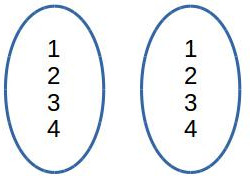
\includegraphics[width=0.3\textwidth]{pics/menge1.jpg} &
  \vtop{\vskip -64pt \vskip -\ht\strutbox 
    \begin{tabular}{lp{4cm}}
      Die linke Mengen wird als Definitions(menge) \\
      bezeichnet, w"ahrend die rechte Menge als \\
      Werte(menge) bezeichnet wird.
    \end{tabular}\vskip -\dp\strutbox }%
\end{tabular}
\\
\begin{tabular}{p{4cm}p{7cm}}
  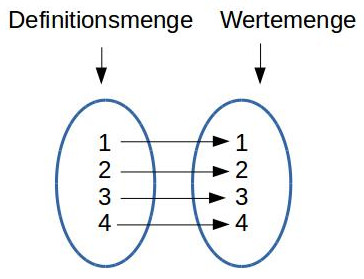
\includegraphics[width=0.3\textwidth]{pics/menge3.jpg} &
  \vtop{\vskip -64pt \vskip -\ht\strutbox 
    \begin{tabular}{lp{4cm}}
      Wie wir bereits wissen, besteht zwischen den \\
      beiden Mengen eine Beziehung. Diese Beziehung \\
      l"asst sich mit Zuordnungspfeilen verdeutlichen. \\
      \\
      $ 1 \mapsto 1 $ \\
      $ \ldots $ \\
      $ 4 \mapsto 4 $
    \end{tabular}\vskip -\dp\strutbox }%
\end{tabular}
\\
\begin{tabular}{p{4cm}p{7cm}}
  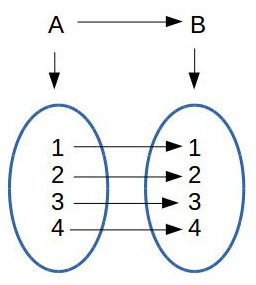
\includegraphics[width=0.3\textwidth]{pics/menge4.jpg} &
  \vtop{\vskip -64pt \vskip -\ht\strutbox 
    \begin{tabular}{lp{4cm}}
      Bei $ f: A \mapsto B $ handelt es sich um eine Funktion, \\
      da jedem Element x der Menge A genau ein Element \\
      y der  Menge B zugeordnet ist. 
    \end{tabular}\vskip -\dp\strutbox }%
\end{tabular}
\\
\begin{tabular}{p{4cm}p{7cm}}
  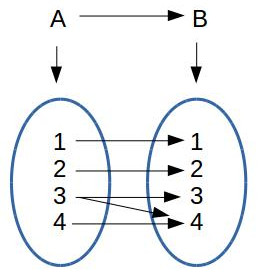
\includegraphics[width=0.3\textwidth]{pics/menge5.jpg} &
  \vtop{\vskip -64pt \vskip -\ht\strutbox 
    \begin{tabular}{lp{4cm}}
      Bei $ f: A \mapsto B $ handelt es sich um keine Funktion, \\
      da dem Element 3 der Menge A zwei Elemente \\
      (3 und 4) der Menge B zugeordnet sind. 4
    \end{tabular}\vskip -\dp\strutbox }%
\end{tabular}
\\
\begin{tabular}{p{4cm}p{7cm}}
  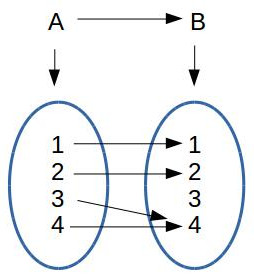
\includegraphics[width=0.3\textwidth]{pics/menge6.jpg} &
  \vtop{\vskip -79pt \vskip -\ht\strutbox 
    \begin{tabular}{lp{4cm}}
    Bei $ f: A \mapsto B $ handelt es sich um eine Funktion, \\
    da jedem Element x der Menge A genau ein Element y der \\
    Menge B zugeordnet ist. \\
    \\
    Dass sich einem Element aus der Menge B zwei Elemente \\
    der Menge A zuordnen lassen, spielt keine Rolle. \\
    Es handelt sich laut Definition trotzdem um eine Funktion.
    \end{tabular}\vskip -\dp\strutbox }%
\end{tabular}
\\
Die Erkenntnisse aus den obigen Beispielen lassen sich folgendermaßen zusammenfassen:
Eine Funktion liegt vor, wenn von jedem Element x der linken Menge (Definitionsmenge)
genau ein Pfeil abgeht.
Von wie vielen Pfeilen ein Element y der rechten Menge (Wertemenge)
getroffen wird, spielt dagegen f"ur die Definition einer Funktion keine Rolle. \\
\\
\textbf{Bezeichnungen und Schreibweisen}
\\
Leider verwenden nicht alle Autoren/Lehrer dieselben Begriffe.
Es ist deshalb notwendig, dass man die alternativen Bezeichnungen
im Hinterkopf beh"alt, um Verwirrungen beim Lesen verschiedener Mathematiktexte
zu vermeiden. \\
\\
Zwei Funktionen sind genau dann identisch, wenn sie in folgenden Teilen "ubereinstimmen:\\
\\
* Funktionsgleichung \\
* Definitionsmenge \\
* Wertemenge \\
\\
Demzufolge sind zwei Funktionen mit gleicher Funktionsgleichung, aber verschiedenen Definitionsmengen
oder verschiedenen Wertemengen, nicht identisch und k"onnen somit unterschiedliche Eigenschaften besitzen. \\
\\
\textbf{Beispiele einer Funktion:} \\
$ y = 2x , \: D = \{ 1, 2, 3 \} , \: W = \{ 2, 4, 8 \} $ \\



\newpage
\chapter{Neuronale Netze}
Tauchen Sie ein, in die wundersame Welt der k"unstlichen Intelligenz. \\
Ich beschreibe hier einen neuralen Netzwerk Simulator, der auch von nicht-technischen Leuten,
einfach zu verstehen ist.
Basierend auf backpropagation'es Lernen f"ur das hier vorgestellte Tool, ist es m"oglich,
Ihren Computer zu trainieren und zu lernen, was Sie von ihm erwarten. \\
Ich m"ochte Ihnen zugleich einen Vorrausblick geben, was uns in naher Zukunft erwartet. \\

\section{Arten von Netzwerken}
Folgende neurale Netzwerke, werde ich hier noch vorstellen:\\
* ein Netzwerk, um die Zahlen 1, 2, und 3 zu erkennen. \\
* ein Netzwerk, um die logische Funktion AND zu verarbeiten. \\
* ein Netzwerk, um die logische Funktion XOE zu verarbeiten. \\

\section{Was sind Neuronale Netzwerke ?}
Expert Definition: \\
Ein neurales Netzwerk ist eine parallel-laufende Informationsstruktur.

\chapter{Sigmoid Funktion}
Eine Sigmoidfunktion, Schwanenhalsfunktion oder S-Funktion ist eine mathematische Funktion mit einem
S-förmigen Graphen.
Oft wird der Begriff Sigmoidfunktion auf den Spezialfall logistische Funktion bezogen,
die durch die Gleichung:\\
{\Large{$sig(t) = \frac{1}{1+e^{-t}} = \frac{e^t}{1 + e^t} = \frac{1}{2}*(1 + \tanh \frac{t}{2})$}}

\begin{figure}[h!]
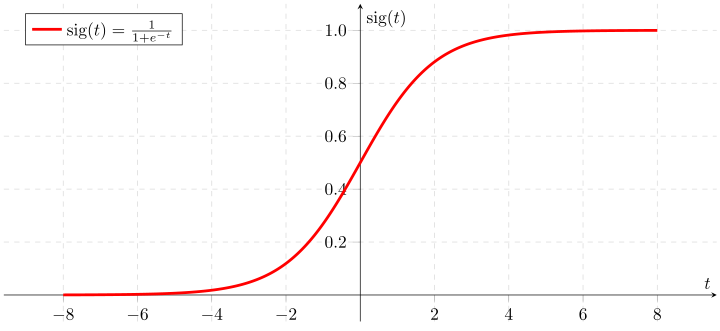
\includegraphics[width=0.7\linewidth]{pics/Sigmoid}
\caption{Graph der Sigmoid-Funktion}
\label{fig:Sigmoid}
\end{figure}


\chapter{Formelsammlung}
Anbei von mir f"ur n"utzliche empfundene Formeln und Schaubilder:

\section{Umrechnungen}
\begin{table}[h!]
\begin{tabular}[t]{|l|l|l|}
\hline
Arbeit   & $1 J = 1 = \frac{W}{s} = 1 Nm$ & -\\
\hline
Leistung & $1 W = 1 * \frac{Nm}{s}$ & $1 PS = 735,49875 W$ \\
\hline
W"arme   & $1 J = 1 * \frac{W}{s}$  & $1 kcal = 4,187 kJ$  \\
         &                          & Wasser: $c = 4,187 \frac{kJ}{kg * K}$\\
\hline
Kraft, Druck &  $1 N = \frac{WA_s}{m}$ ;  & 1 kp = 9,81 N \\
             &  $1 bar = 10^5 * \frac{N}{m^2}$ & \\
\hline
Geschwindigkeit & $1 * \frac{m}{s} = 3,6 * \frac{km}{h}$ & -\\
\hline
Magnetisches Feld & $1 Wb = 1 * V_s$ ; & $\mu_0 = 4 * \pi * 10^{-7} \frac{V_s}{Am}$ \\
                  &                             & \\
                  & $1 T = 1 * \frac{V_s}{m^2}$ & $\mu_0 = 1,257 * 10^{-6} \frac{V_s}{Am}$\\
\hline
Spule & $1 H = 1 * \frac{Vs}{A}$ & \\
\hline
Elektrisches Feld & - &\\
Kondensator & $1 F = 1 * \frac{A_s}{V} = 1 * \frac{s}{\Omega}$ & $s_0 = 8,854 * 10^{-12} \frac{A_s}{Vm}$ \\
\hline
\end{tabular}
\end{table}


\section{mathematische Formeln}
\begin{tabular}[t]{| p{5cm} | p{4cm} | p{2cm} |}
\hline
\begin{minipage}{0.52\textwidth}
  \textbf{Satz des Pythagoras}\\
  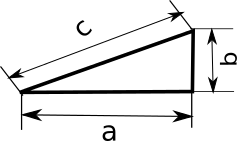
\includegraphics[width=0.385\textwidth, height=0.100\textheight]{pics/flow7284.png} \\
\end{minipage}
&
\begin{minipage}{0.52\textwidth}
a = Ankathete  \\
b = Gegenkathete \\
c = Hypotenuse \\
\end{minipage}
&
\begin{minipage}{0.51\textwidth}
$c^2 = a^2 + b^2$
\end{minipage}
\\
\hline
\begin{minipage}{0.52\textwidth}
  \textbf{Trigonometrische \\ Funktionen}\\
  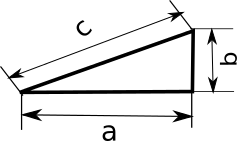
\includegraphics[width=0.385\textwidth, height=0.100\textheight]{pics/flow7284.png}
\end{minipage}
&
\begin{minipage}{0.52\textwidth}
a = Ankathete  \\
b = Gegenkathete \\
c = Hypotenuse \\
\end{minipage}
&
\begin{minipage}{0.52\textwidth}
sin $\mathbb{\varphi} = b/c$ \\
cos $\mathbb{\varphi} = a/c$ \\
tan $\mathbb{\varphi} = b/a$ \\
\end{minipage}
\\
\hline
\end{tabular}



% Anhang -----------------------------------------------------------------------
%   Die Inhalte des Anhangs werden analog zu den Kapiteln inkludiert.
%   Dies geschieht in der Datei "Anhang.tex".
% ------------------------------------------------------------------------------
\newpage
\begin{appendix}
    \clearpage
     \chapter{Anhang}
    \label{sec:Anhang}
\end{appendix}



\end{document}

